%\begin{frame}
%  \frametitle{Hybrid $S_N$-Diffusion Method: Preliminary Results}
%  \textbf{Illustration of the Hybrid Method With Case 0} \\
%  \begin{columns}
%    \column[t]{5.5cm}
%    \textbf{Problem Description}
%    \begin{itemize}
%      \item 1-D, two-region system consisting of:
%      \begin{itemize}
%        \item 0.5-cm thick control rod region
%        \item 19.5-cm thick homogenized mixture of molten fuel salt and graphite moderator
%      \end{itemize}
%      \item Material compositions from the Molten Salt Reactor Experiment (MSRE)
%      \item Two-group constants are sampled at 900 K and generated using OpenMC
%    \end{itemize}
%    \column[t]{5.5cm}
%    \begin{figure}[htb!]
%      \centering
%      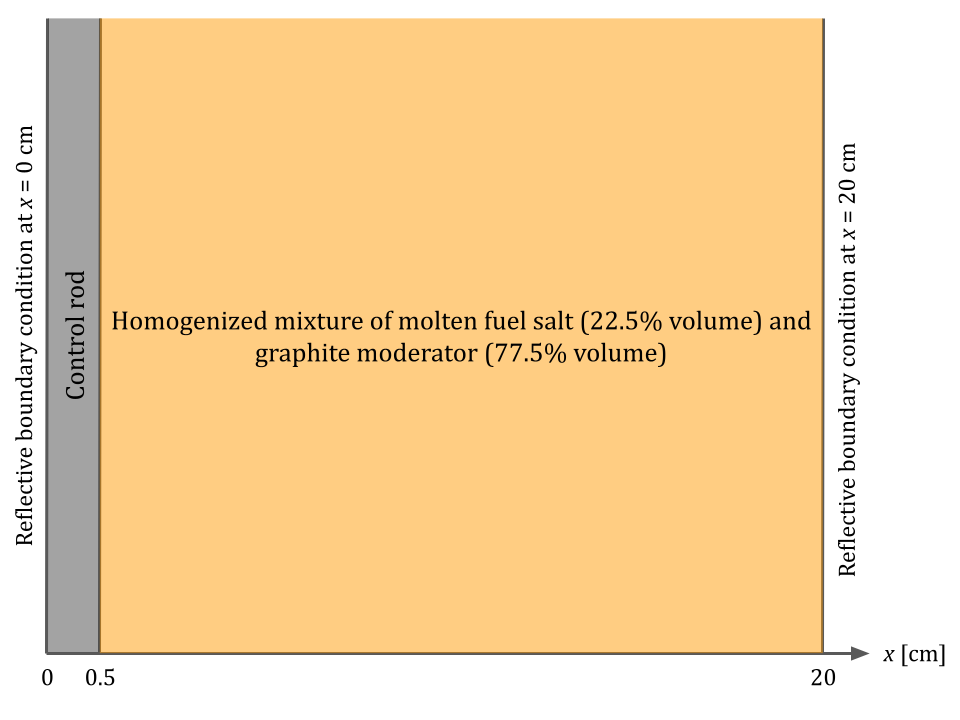
\includegraphics[width=\columnwidth]{../images/case-0-geometry}
%      \caption{Case 0 problem geometry.}
%      \label{fig:case-0-geom}
%    \end{figure}
%  \end{columns}
%\end{frame}
%
%\begin{frame}
%  \frametitle{Hybrid $S_N$-Diffusion Method: Preliminary Results}
%  \textbf{Illustration of the Hybrid Method With Case 0}
%  \vspace{.3cm}
%
%  I solved for the neutron flux in Case 0 using the following set of numerical solvers:
%  \begin{enumerate}
%    \item Neutron diffusion solver with $P_1$-based diffusion coefficients generated directly from
%      the group constants generation step with OpenMC
%    \item $S_N$ neutron transport solver with $N=8$ and up to 2nd-order Legendre expansions of
%      scattering cross sections
%    \item Neutron diffusion solver with SVDCs generated from the prior $S_8$ flux solution
%    \item Hybrid $S_N$-Diffusion solver with $\Omega^d_1$ spanning from $x=0$ cm to $x=17.5$ cm
%  \end{enumerate}
%
%  The neutron diffusion and $S_N$ solvers are implemented in Python using the finite difference
%  method and diamond difference method, respectively.
%\end{frame}
%
%\begin{frame}
%  \frametitle{Hybrid $S_N$-Diffusion Method: Preliminary Results}
%  \textbf{Case 0 Results}
%  \begin{figure}
%    \centering
%    \begin{subfigure}[b]{.49\textwidth}
%      \centering
%      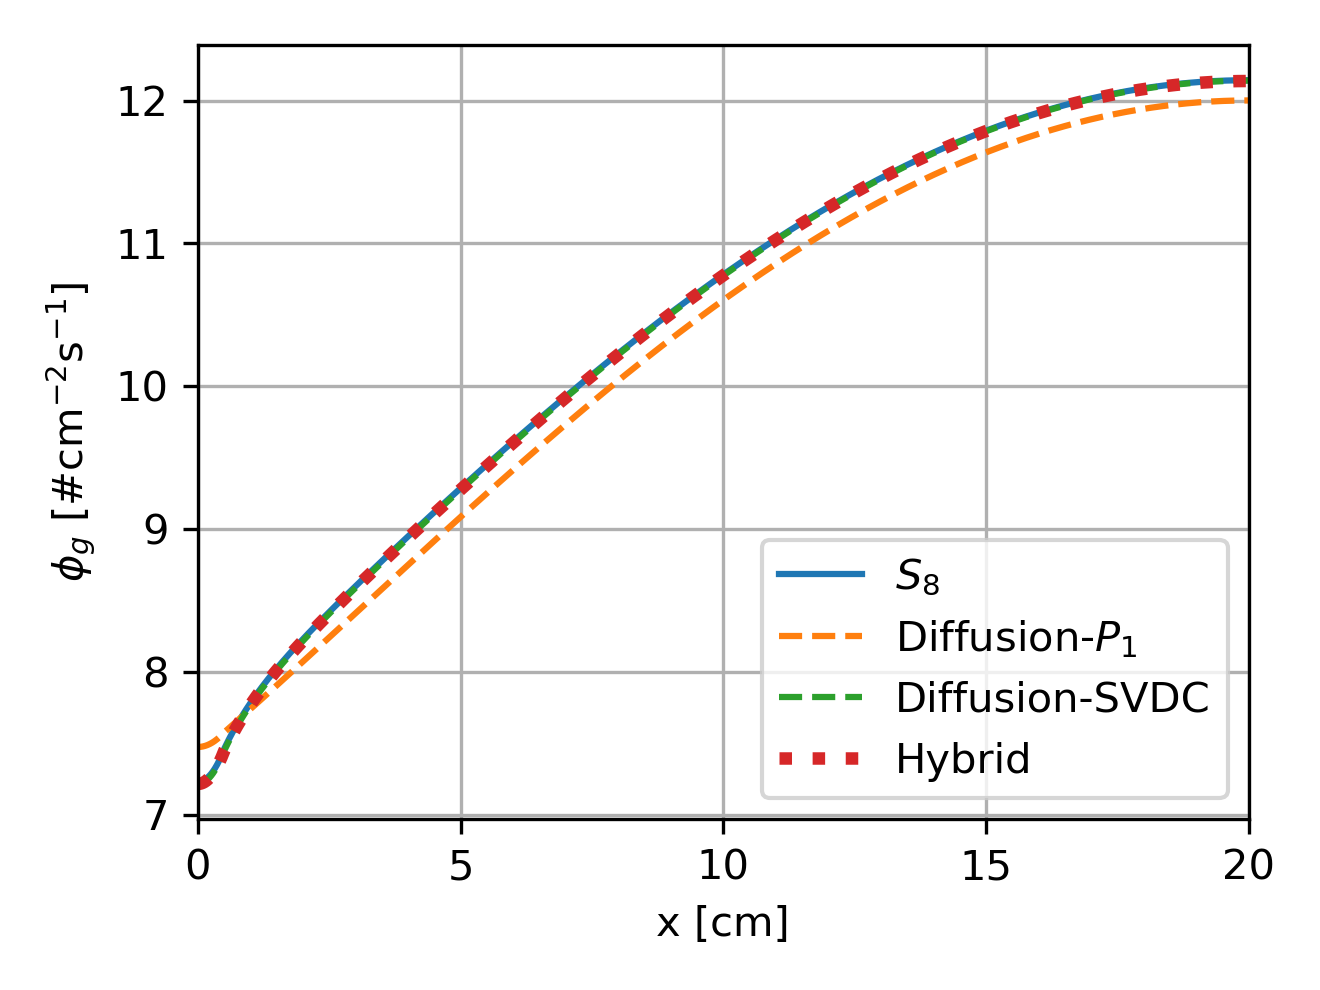
\includegraphics[width=\textwidth]{../images/case-0-group-1-hybrid-flux}
%      \caption{Group 1}
%      \label{fig:c0g1hf}
%    \end{subfigure}
%    \hfill
%    \begin{subfigure}[b]{.49\textwidth}
%      \centering
%      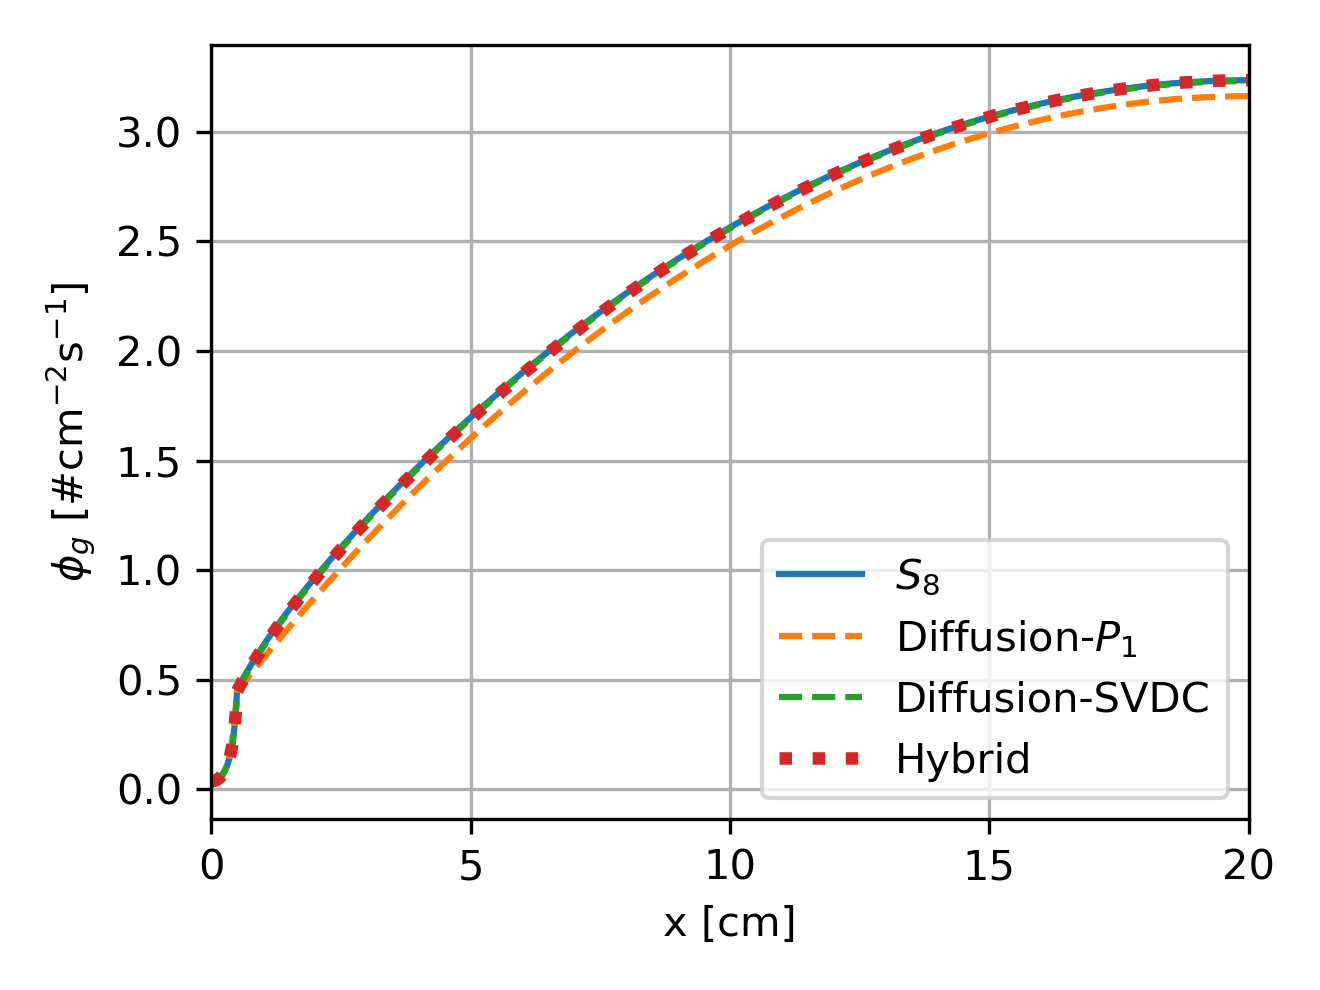
\includegraphics[width=\textwidth]{../images/case-0-group-2-hybrid-flux}
%      \caption{Group 2}
%      \label{fig:c0g2hf}
%    \end{subfigure}
%    \caption{Neutron group 1 and 2 flux distributions from the diffusion, $S_8$, reference
%    \gls{SVDC}, and hybrid methods for Case 0.}
%  \end{figure}
%\end{frame}
%
%\begin{frame}
%  \frametitle{Hybrid $S_N$-Diffusion Method: Preliminary Results}
%  \textbf{Case 0 Results}
%  \begin{figure}
%    \centering
%    \begin{subfigure}[b]{.49\textwidth}
%      \centering
%      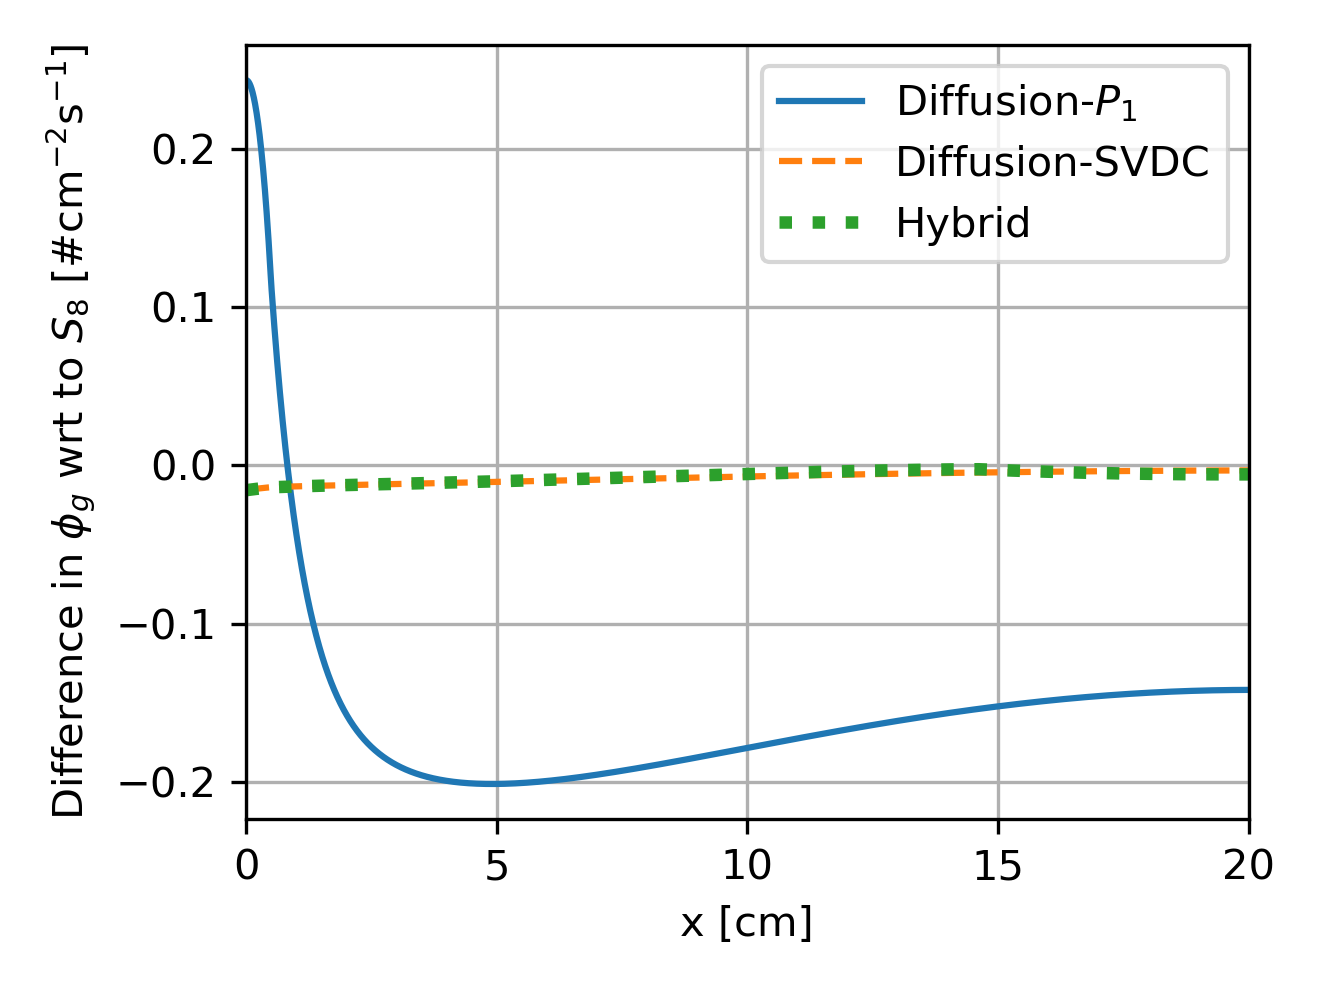
\includegraphics[width=\textwidth]{../images/case-0-group-1-hybrid-flux-diff}
%      \caption{Group 1}
%      \label{fig:c0g1hfdiff}
%    \end{subfigure}
%    \hfill
%    \begin{subfigure}[b]{.49\textwidth}
%      \centering
%      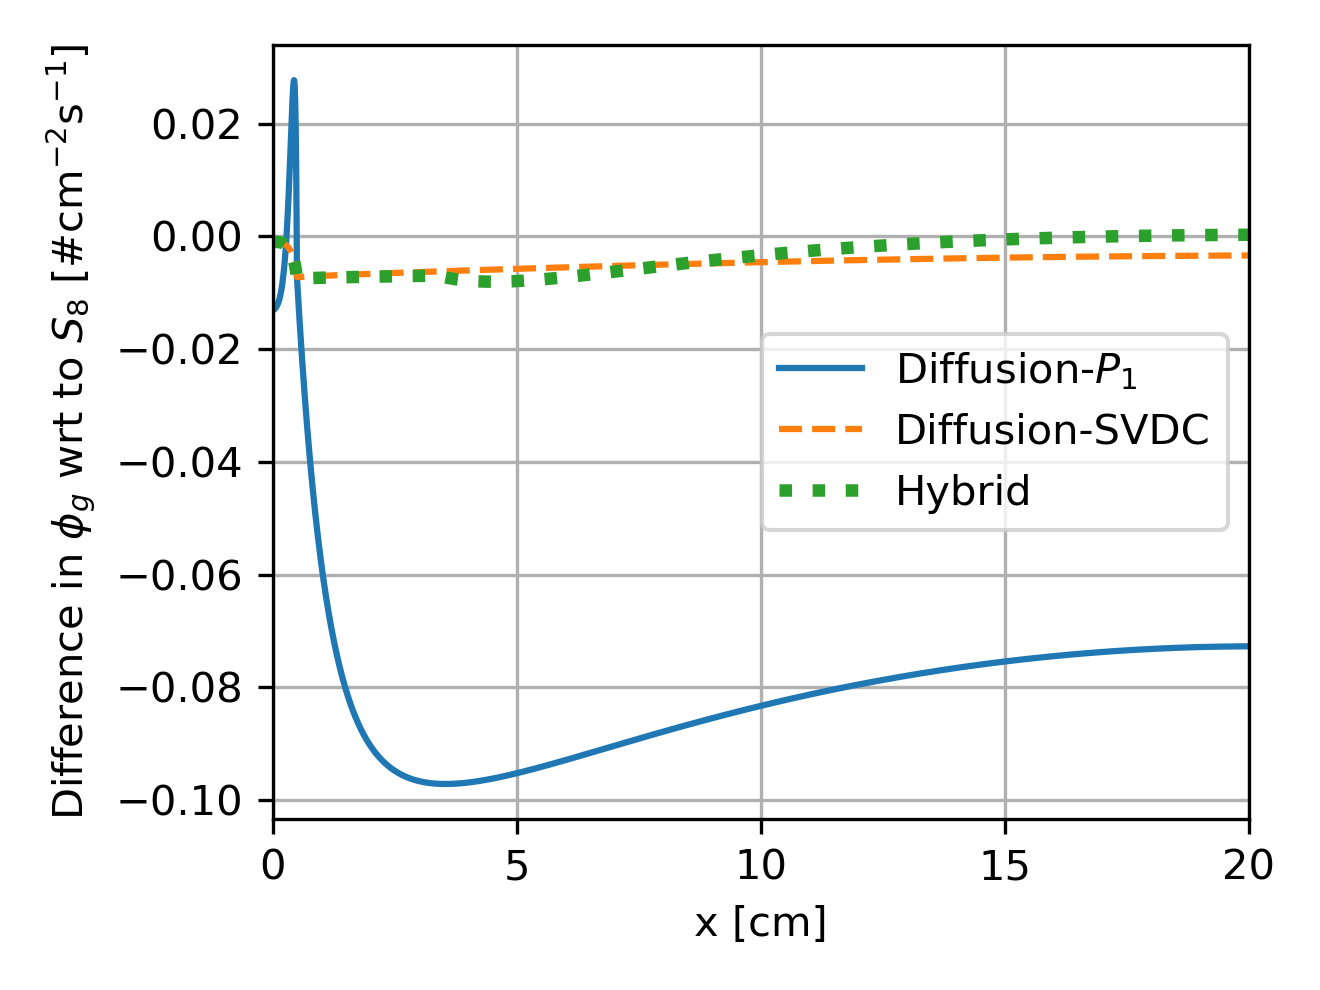
\includegraphics[width=\textwidth]{../images/case-0-group-2-hybrid-flux-diff}
%      \caption{Group 2}
%      \label{fig:c0g2hfdiff}
%    \end{subfigure}
%    \caption{Difference in neutron group 1 and 2 flux distributions from the diffusion,
%    diffusion-\gls{SVDC}, and hybrid methods with respect to the $S_8$ flux distribution for Case 0.}
%    \label{fig:c0hfdiff}
%  \end{figure}
%\end{frame}
%
%\begin{frame}
%  \frametitle{Hybrid $S_N$-Diffusion Method: Preliminary Results}
%  \textbf{Case 0 Results}
%  \begin{table}
%    \centering
%    \caption{Multiplication factor $k$ estimates from the $S_8$, diffusion-$P_1$,
%    diffusion-\gls{SVDC}, and hybrid solvers and the absolute difference relative to the $S_8$
%    estimate.}
%    \begin{tabular}{l S S}
%      \toprule
%      Solver type & {$k$} & {$k-k_{S_8}$} \\
%      \midrule
%      $S_8$ & 0.62736 & {-} \\
%      Diffusion-$P_1$ & 0.60890 & -0.01846 \\
%      Diffusion-\gls{SVDC} & 0.62750 & +0.00013 \\
%      Hybrid & 0.62774 & +0.00038 \\
%      \bottomrule
%    \end{tabular}
%    \label{table:c0k}
%  \end{table}
%\end{frame}
%
%\begin{frame}
%  \frametitle{Hybrid $S_N$-Diffusion Method: Preliminary Results}
%  \textbf{Case 0 Results}
%  \begin{figure}[htb!]
%    \centering
%    \begin{subfigure}[b]{.49\textwidth}
%      \centering
%      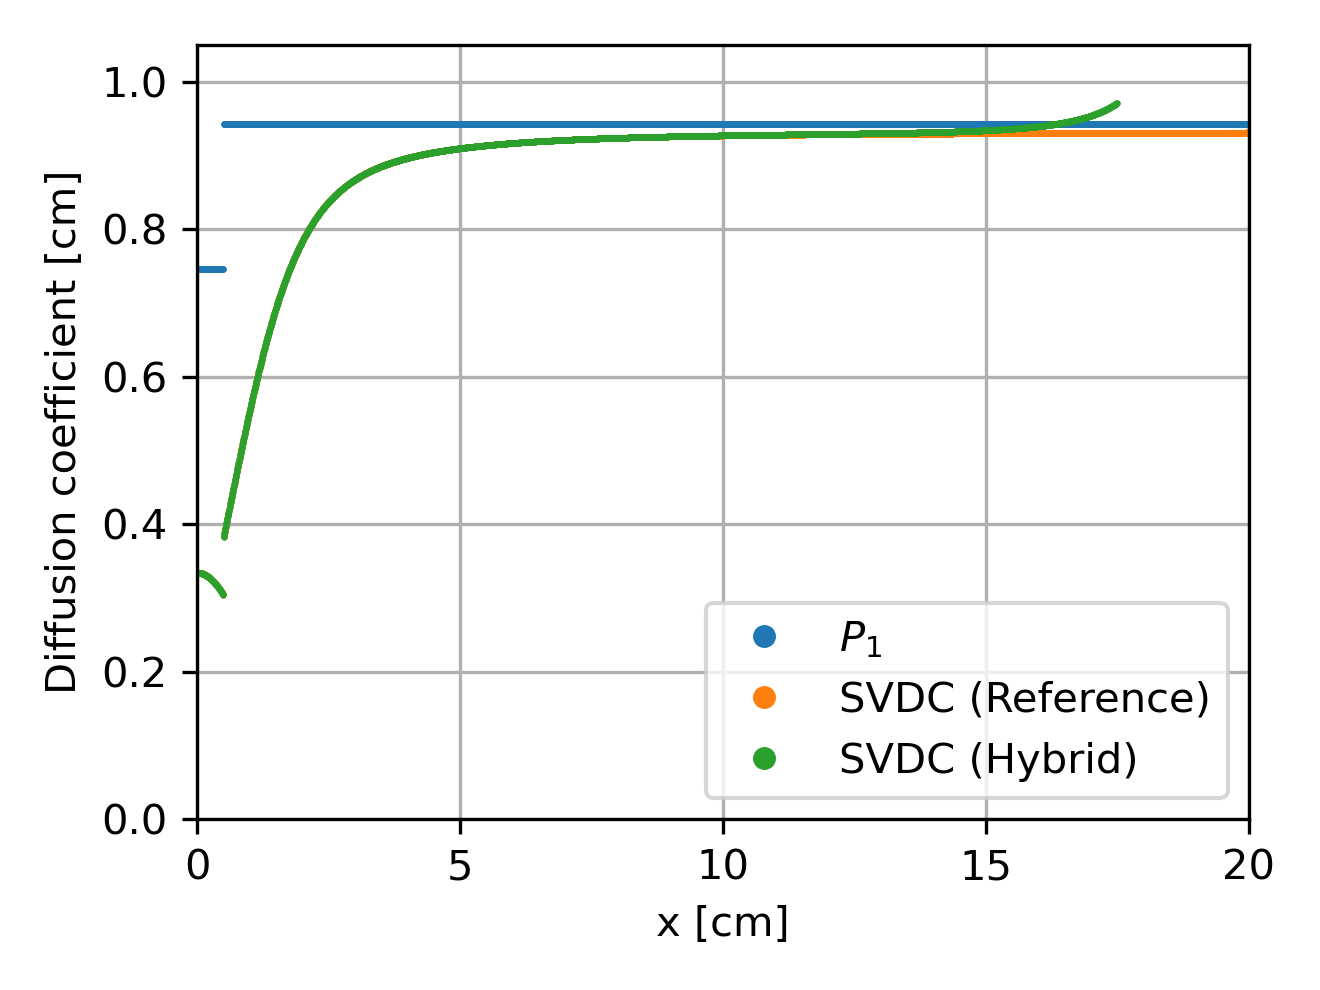
\includegraphics[width=\textwidth]{../images/case-0-group-1-hybrid-diffcoef}
%      \caption{Group 1}
%      \label{fig:c0g1hd}
%    \end{subfigure}
%    \hfill
%    \begin{subfigure}[b]{.49\textwidth}
%      \centering
%      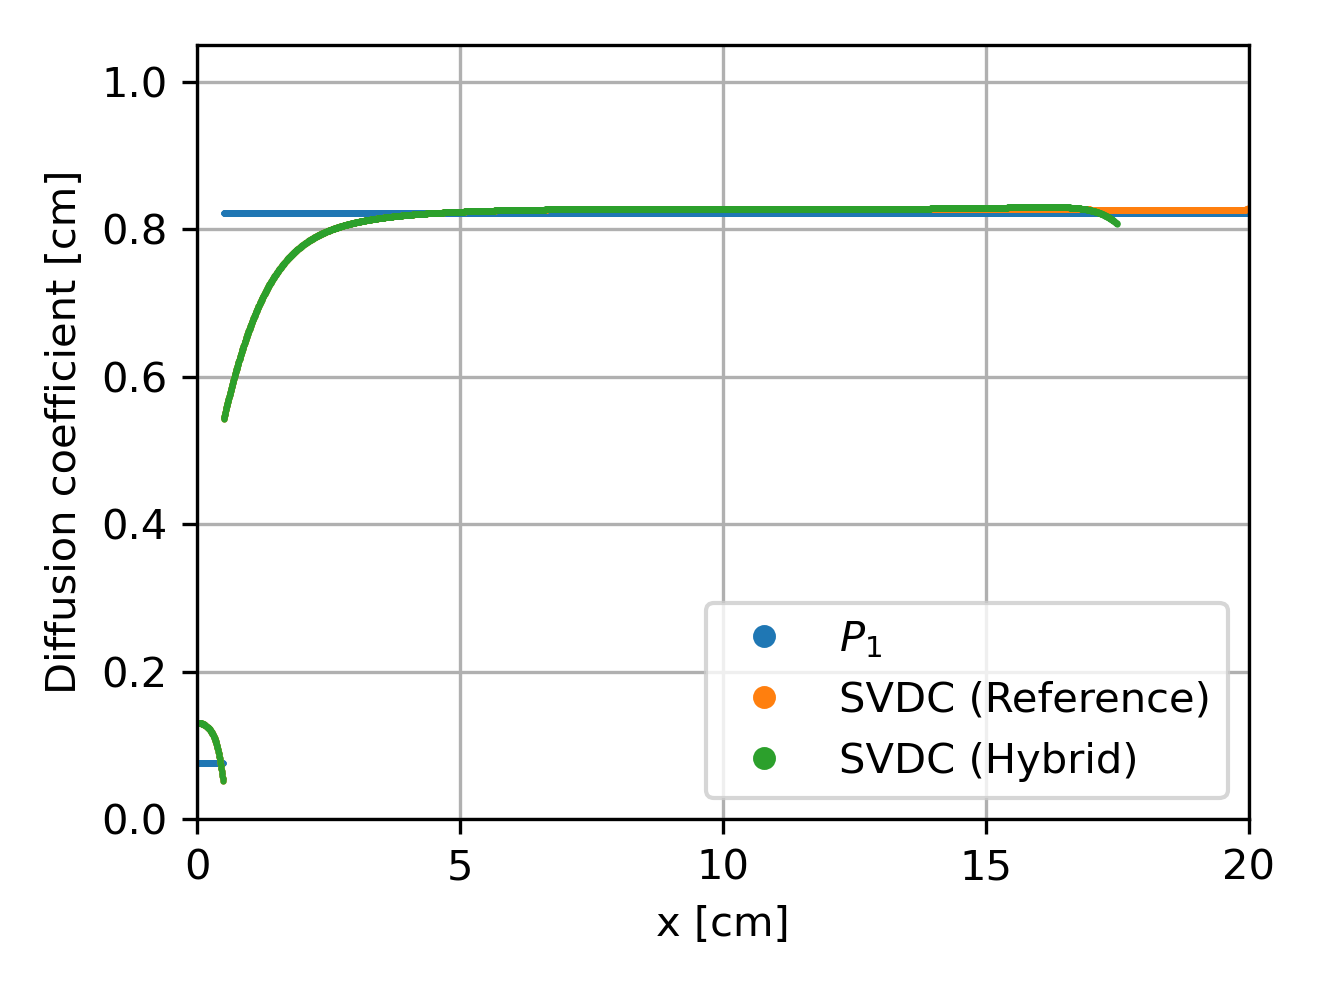
\includegraphics[width=\textwidth]{../images/case-0-group-2-hybrid-diffcoef}
%      \caption{Group 2}
%      \label{fig:c0g2hd}
%    \end{subfigure}
%    \caption{$P_1$-based flux-limited diffusion coefficient and \gls{SVDC} spatial distribution for
%    Case 0. The \gls{SVDC} distributions were generated from the reference $S_8$ (``SVDC'') and the
%    hybrid (``Hybrid'') calculations.}
%    \label{fig:c0hd}
%  \end{figure}
%\end{frame}
%
%\begin{frame}
%  \frametitle{Hybrid $S_N$-Diffusion Method: Preliminary Results}
%  \textbf{Case 0 Discussion}
%  \begin{itemize}
%    \item The hybrid method automatically determines the buffer zone size by comparing the SVDCs
%      to the $P_1$ diffusion coefficient values.
%    \item The hybrid method converges rapidly within two outer iterations.
%    \item The required size of $V_1$ for Case 0 is large because the control rod region is
%      the only significant source of influence on the neutron flux.
%    \item $V_1$ is smaller for more realistic reactor systems which are more heterogeneous
%      and have vacuum boundary conditions.
%  \end{itemize}
%\end{frame}

\begin{frame}
  \frametitle{Hybrid $S_N$-Diffusion Method: Preliminary Results}
  \textbf{1-D Test Cases}
  \begin{figure}[htb!]
    \centering
    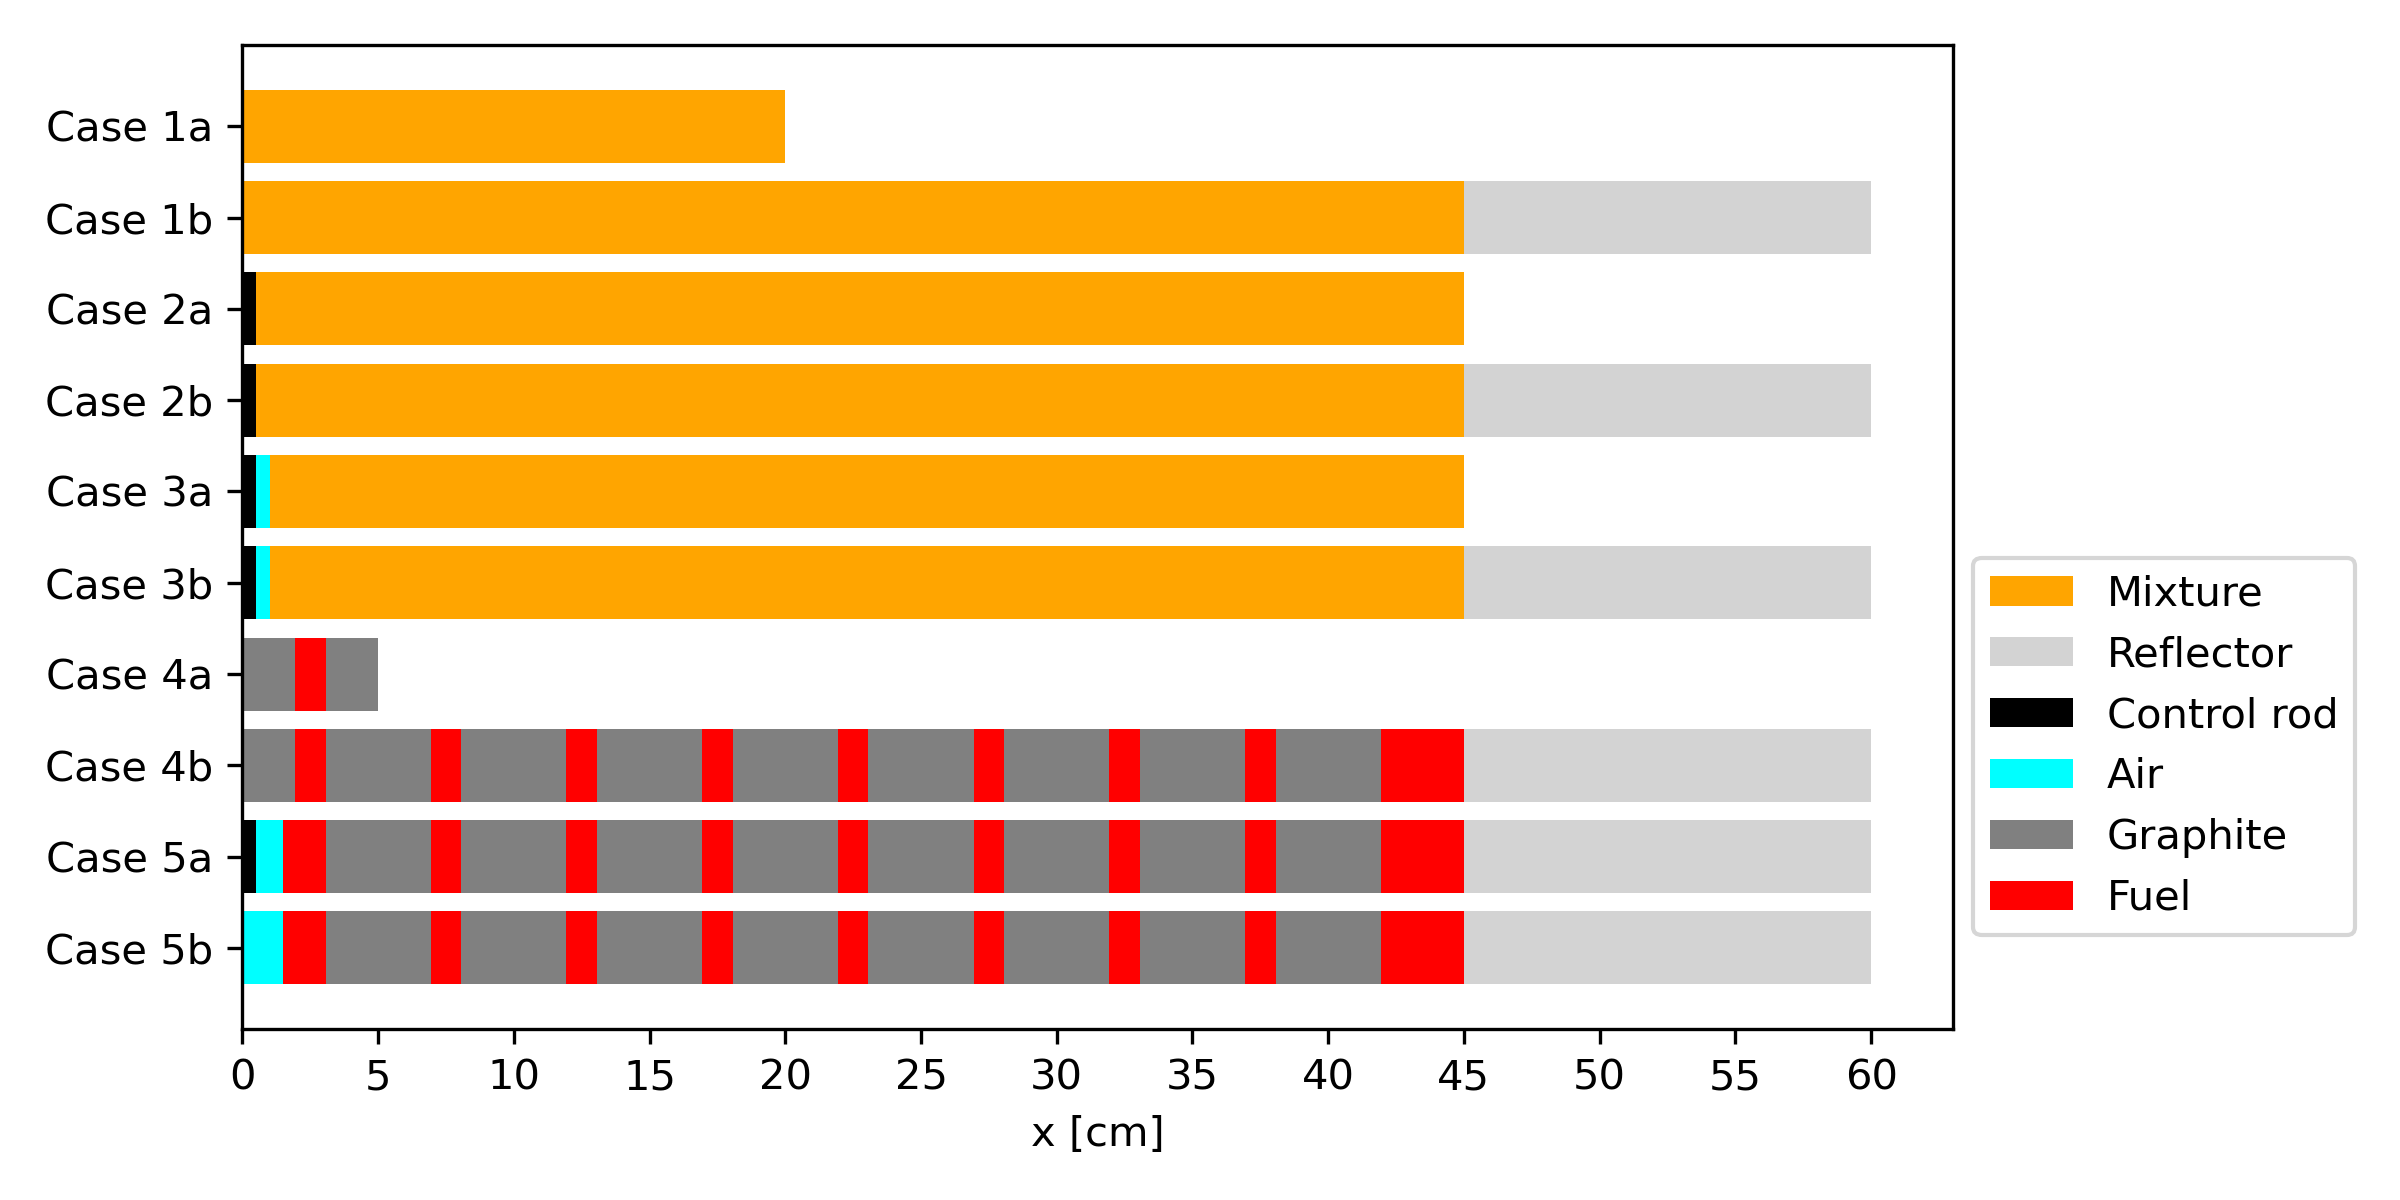
\includegraphics[width=\columnwidth]{../images/case-geometry}
    \caption{Geometries of the 1-D test cases. All geometries
      have reflective boundary conditions on the boundary at $x=0$ cm. The right-side boundaries are
      reflective for Cases 1a, 2a, 3a, and 4a, and vacuum for Cases 1b, 2b, 3b, 4b, 5a, and 5b.}
    \label{fig:case-geom}
  \end{figure}
\end{frame}

\begin{frame}
  \frametitle{Hybrid $S_N$-Diffusion Method: Preliminary Results}
  \textbf{1-D Test Case Problem Setup}
  \begin{itemize}
    \item Material compositions derived from the MSRE design
    \item Four neutron energy groups
      \begin{itemize}
        \item Bounded at $E=[10^{-5}, 10^0, 10^2, 10^5, 10^8]$ eV
      \end{itemize}
    \item Group constants generated using OpenMC with up to 2nd-order Legendre expansions of the
      scattering matrices
  \end{itemize}
\end{frame}

\begin{frame}
  \frametitle{Hybrid $S_N$-Diffusion Method: Preliminary Results}
  \textbf{1-D Test Case Numerical Solvers}
  \vspace{.2cm}

  The neutron diffusion and $S_N$ solvers are implemented in Python using the finite difference
  method and diamond difference method, respectively.
  \vspace{.2cm}

  I solved for the neutron fluxes using the following set of numerical solvers:
  \begin{enumerate}
    \item OpenMC Monte Carlo neutron transport solver in continuous energy mode
    \item OpenMC Monte Carlo neutron transport solver in multigroup mode
    \item Neutron diffusion solver with $P_1$-based diffusion coefficients generated directly from
      the group constants generation step with OpenMC
    \item $S_N$ neutron transport solver with $N=8$ ($S_N$ calculation in $V_0$)
    \item Hybrid $S_N$-Diffusion solver with $N=8$ ($S_N$ subcalculation in $V_1$)
  \end{enumerate}
\end{frame}

\begin{frame}
  \frametitle{Hybrid $S_N$-Diffusion Method: Preliminary Results}
  \textbf{Simulation Parameters}
  \begin{table}
    \centering
    \footnotesize
    \caption{Simulation parameters applied to the neutron diffusion, $S_N$, and Hybrid
    $S_N$-Diffusion methods.}
    \begin{tabular}{c c c c}
      \toprule
      Parameter & $S_N$ Transport & Neutron Diffusion & Hybrid $S_N$-Diffusion \\
      \midrule
      Mesh size, $\Delta x$ [cm]        & 0.0125    & 0.0125    & 0.0125 \\[.2cm]
      \multirow{3}{*}{Convergence tolerance, $tol$}
                                        &           &           & Diffusion: $10^{-6}$ \\
                                        & $10^{-7}$ & $10^{-6}$ & $S_N$: $10^{-5}$ \\
                                        &           &           & Outer: $10^{-3}$ \\[.2cm]
      Discrete ordinates, $N$           & 8         & N/A       & 8 \\
      Highest moment of $\Sigma^{g'\rightarrow g}_s$, $L$
                                        & 2         & N/A       & 2 \\
      \bottomrule
    \end{tabular}
    \label{table:param}
  \end{table}
\end{frame}

%\begin{frame}
%  \frametitle{Hybrid $S_N$-Diffusion Method: Preliminary Results}
%  \textbf{Test Case Results}
%  \begin{table}
%    \centering
%    \scriptsize
%    \caption{Multiplication factor $k$ estimates for Cases 1a, 1b, 2a, 2b, 3a, and 3b.}
%    \begin{tabular}{c S[table-format=1.5(2)] S[table-format=1.5(2)] S[table-format=1.5(2)]
%    S[table-format=1.5(2)] S[table-format=1.5(2)] S[table-format=1.5(2)]}
%      \toprule
%      \multirow{2}{*}{\textbf{Method}} &
%      \multicolumn{6}{c}{\textbf{Multiplication factor,} $\bm{k}$} \\
%      \cmidrule{2-7}
%      & {\textbf{Case 1a}} & {\textbf{Case 1b}} & {\textbf{Case 2a}} &
%      {\textbf{Case 2b}} & {\textbf{Case 3a}} & {\textbf{Case 3b}} \\
%      \midrule
%      OpenMC-CE & 1.60033(56) & 1.16749(60) & 1.20666(66) & 0.69499(47) & 1.19908(63) & 0.68565(53)\\
%      OpenMC-MG & 1.60015(33) & 1.18104(54) & 1.20570(66) & 0.70539(50) & 1.19976(48) & 0.69730(50)\\
%      $S_8$     & 1.60035     & 1.18068     & 1.20596     & 0.70470     & 1.19968     & 0.69652    \\
%      Diffusion & 1.60036     & 1.17932     & 1.19709     & 0.69274     & 1.19064     & 0.68450    \\
%      Hybrid    & {N/A}       & {N/A}       & 1.20630     & 0.70387     & 1.20004     & 0.69568    \\
%      \bottomrule
%    \end{tabular}
%    \label{table:ck1}
%  \end{table}
%  %
%  \begin{table}
%    \centering
%    \scriptsize
%    \caption{Multiplication factor $k$ estimates for Cases 4a, 4b, 5a, and 5b.}
%    \begin{tabular}{c S[table-format=1.5(2)] S[table-format=1.5(2)] S[table-format=1.5(2)]
%      S[table-format=1.5(2)]}
%      \toprule
%      \multirow{2}{*}{\textbf{Method}} &
%      \multicolumn{4}{c}{\textbf{Multiplication factor,} $\bm{k}$} \\
%      \cmidrule{2-5}
%      & {\textbf{Case 4a}} & {\textbf{Case 4b}} & {\textbf{Case 5a}} &
%      {\textbf{Case 5b}} \\
%      \midrule
%      OpenMC-CE & 1.64506(53) & 1.19116(63) & 0.70352(64) & 1.16832(58) \\
%      OpenMC-MG & 1.64355(37) & 1.20738(63) & 0.71396(50) & 1.18204(53) \\
%      $S_8$     & 1.64376     & 1.20744     & 0.71379     & 1.18218     \\
%      Diffusion & 1.64355     & 1.20811     & 0.70524     & 1.18274     \\
%      Hybrid    & {N/A}       & {N/A}       & 0.71673     & {N/A}       \\
%      \bottomrule
%    \end{tabular}
%    \label{table:ck2}
%  \end{table}
%\end{frame}

\begin{frame}
  \frametitle{Hybrid $S_N$-Diffusion Method: Preliminary Results}
  \textbf{Differences in Neutron Multiplication Factor, $k$}
  \begin{columns}
    \column{12cm}
  \begin{table}[htb!]
    \centering
    \scriptsize
    \caption{Differences in $k$ estimates for 2b, 3a, 3b, and 5a for the $S_8$ neutron
      transport, neutron diffusion, and Hybrid $S_N$-Diffusion methods relative to OpenMC-MG.}
    \begin{tabular}{c S[table-format=+1.5(2)] S[table-format=+1.5(2)] S[table-format=+1.5(2)]
        S[table-format=+1.5(2)] S[table-format=+1.5(2)]}
      \toprule
      \multirow{2}{*}{\textbf{Method}} & \multicolumn{5}{c}{$\bm{k-k_{MG}}$} \\
      \cmidrule{2-6}
      & {\textbf{Case 2a}} & {\textbf{Case 2b}} & {\textbf{Case 3a}} & {\textbf{Case 3b}}
      & {\textbf{Case 5a}} \\
      \midrule
      $S_8$     & +0.00026(66) & -0.00069(50) & -0.00008(48) & -0.00078(50) & -0.00017(50) \\
      Diffusion & -0.00861(66) & -0.01265(50) & -0.00912(48) & -0.01280(50) & -0.00872(50) \\
      Hybrid    & +0.00060(66) & -0.00152(50) & +0.00028(48) & -0.00162(50) & +0.00070(50) \\
      \bottomrule
    \end{tabular}
    \label{table:ckdiff1}
  \end{table}
\end{columns}
\end{frame}

%\begin{frame}
%  \frametitle{Hybrid $S_N$-Diffusion Method: Preliminary Results}
%  \textbf{Test Case Results}
%  \begin{table}
%    \centering
%    \footnotesize
%    \caption{Control rod worths calculated as changes in the reactivity between Case 5a and 5b for
%      the OpenMC continuous-energy and multigroup mode calculations, and the $S_8$ neutron transport,
%    neutron diffusion, and Hybrid $S_N$-Diffusion methods.}
%    \begin{tabular}{c S}
%      \toprule
%      \multirow{2}{*}{\textbf{Method}} & {\textbf{Control rod worth}} \\
%                                       & {$\bm{\rho_{(5b)}-\rho_{(5a)}}$} \\
%      \midrule
%      OpenMC-CE & 0.56549(213) \\
%      OpenMC-MG & 0.55464(176) \\
%      $S_8$     & 0.55507 \\
%      Diffusion & 0.57246 \\
%      Hybrid    & 0.54974 \\
%      \bottomrule
%    \end{tabular}
%    \label{table:rod-worth}
%  \end{table}
%  The hybrid method generates improved control rod worth estimates over the standard neutron
%  diffusion method.
%\end{frame}

\begin{frame}
  \frametitle{Hybrid $S_N$-Diffusion Method: Preliminary Results}
  \begin{columns}
    \column{8cm}
    \begin{figure}
      \centering
      \begin{subfigure}[t]{.45\textwidth}
        \centering
        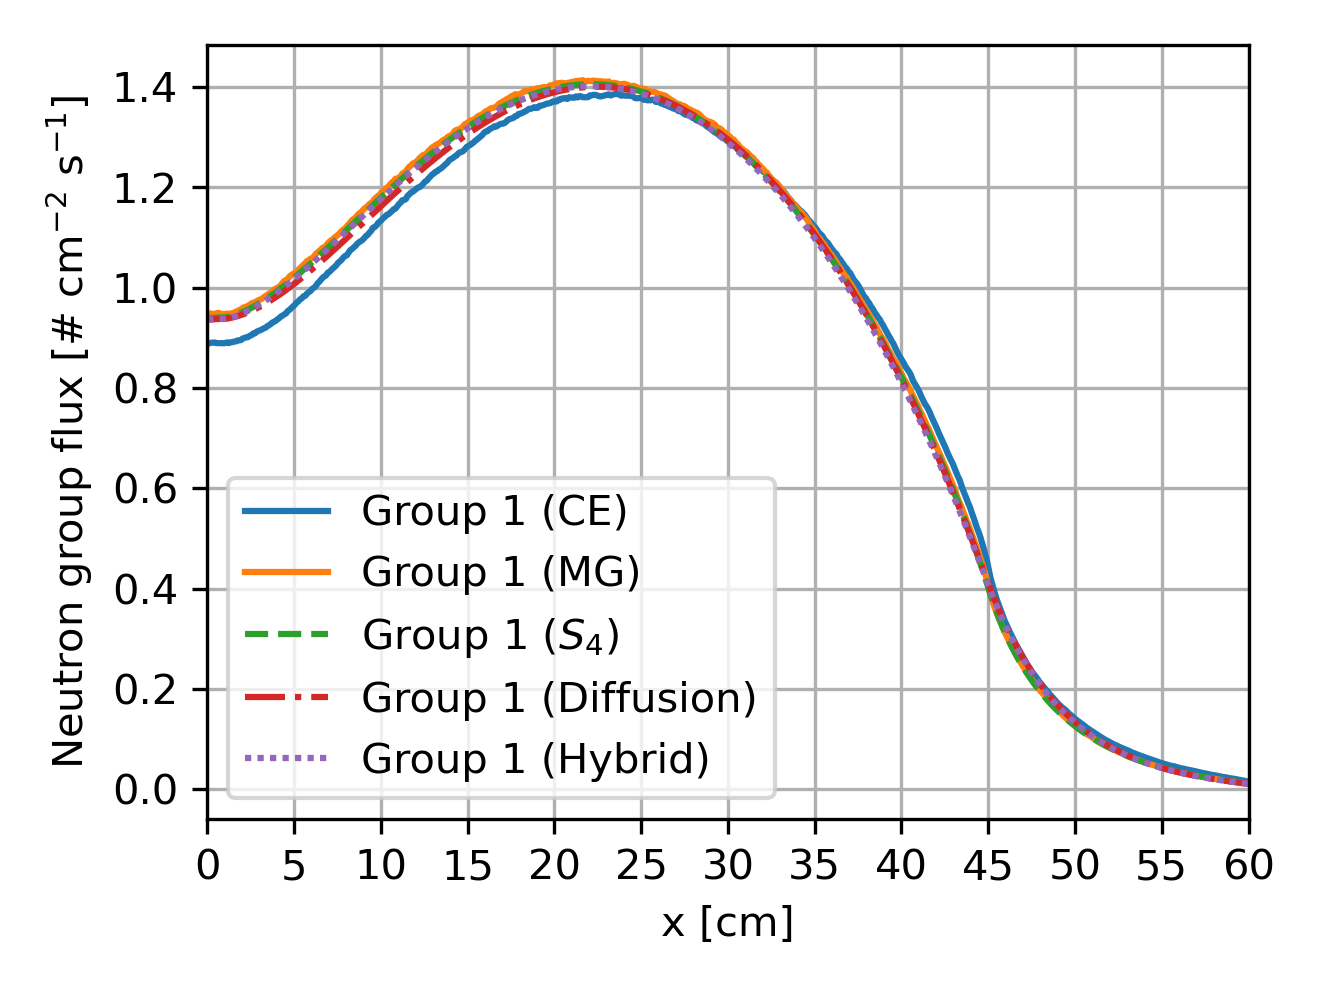
\includegraphics[width=\textwidth]{../images/case-3b-group-1-flux}
        \label{fig:c3bg1}
      \end{subfigure}
      \begin{subfigure}[t]{.45\textwidth}
        \centering
        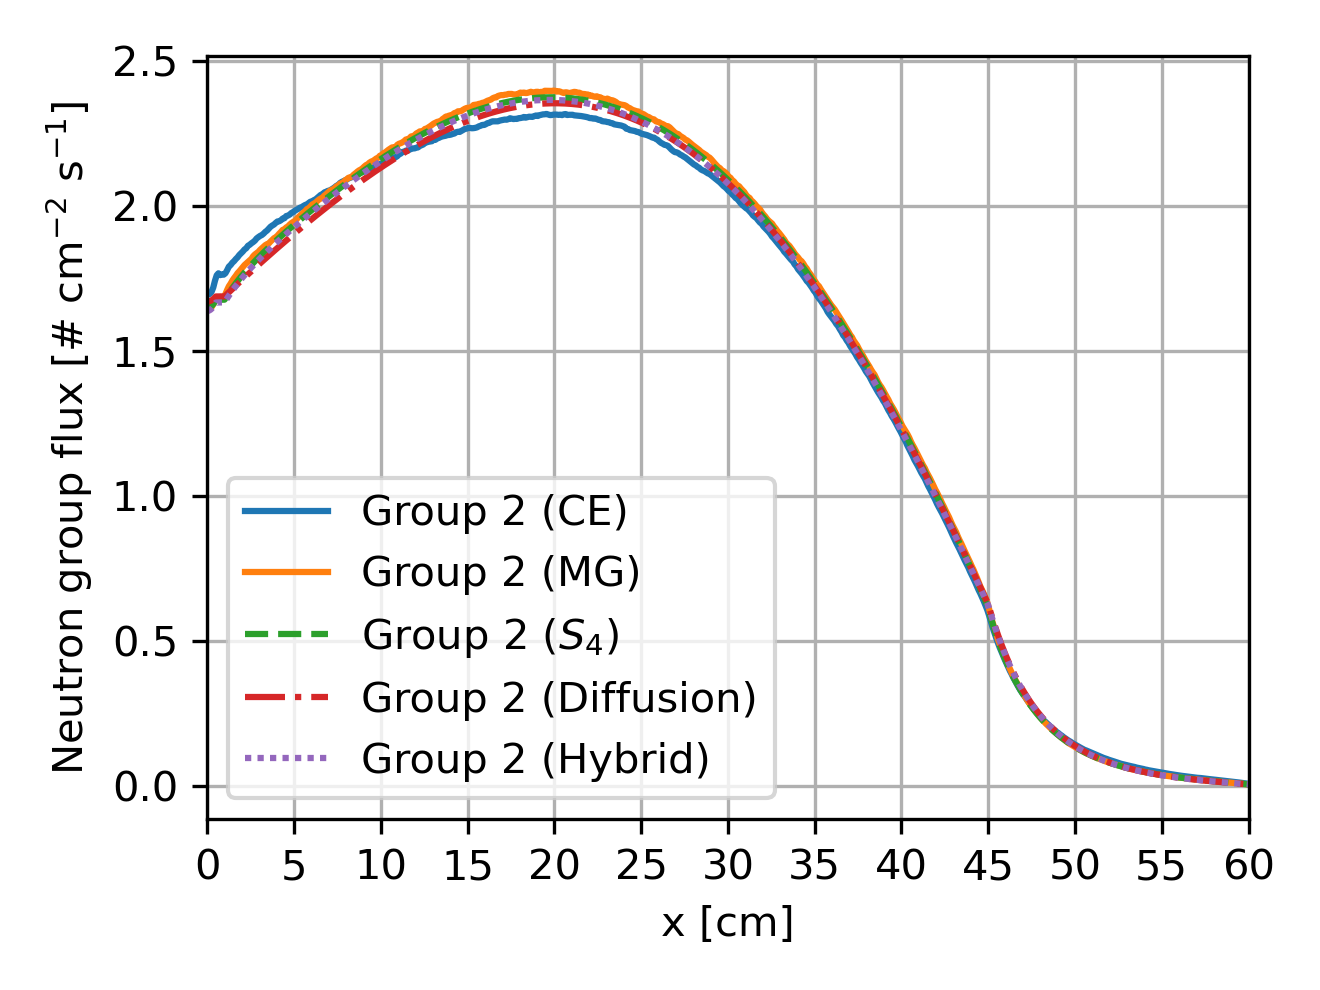
\includegraphics[width=\textwidth]{../images/case-3b-group-2-flux}
        \label{fig:c3bg2}
      \end{subfigure}
      \begin{subfigure}[t]{.45\textwidth}
        \centering
        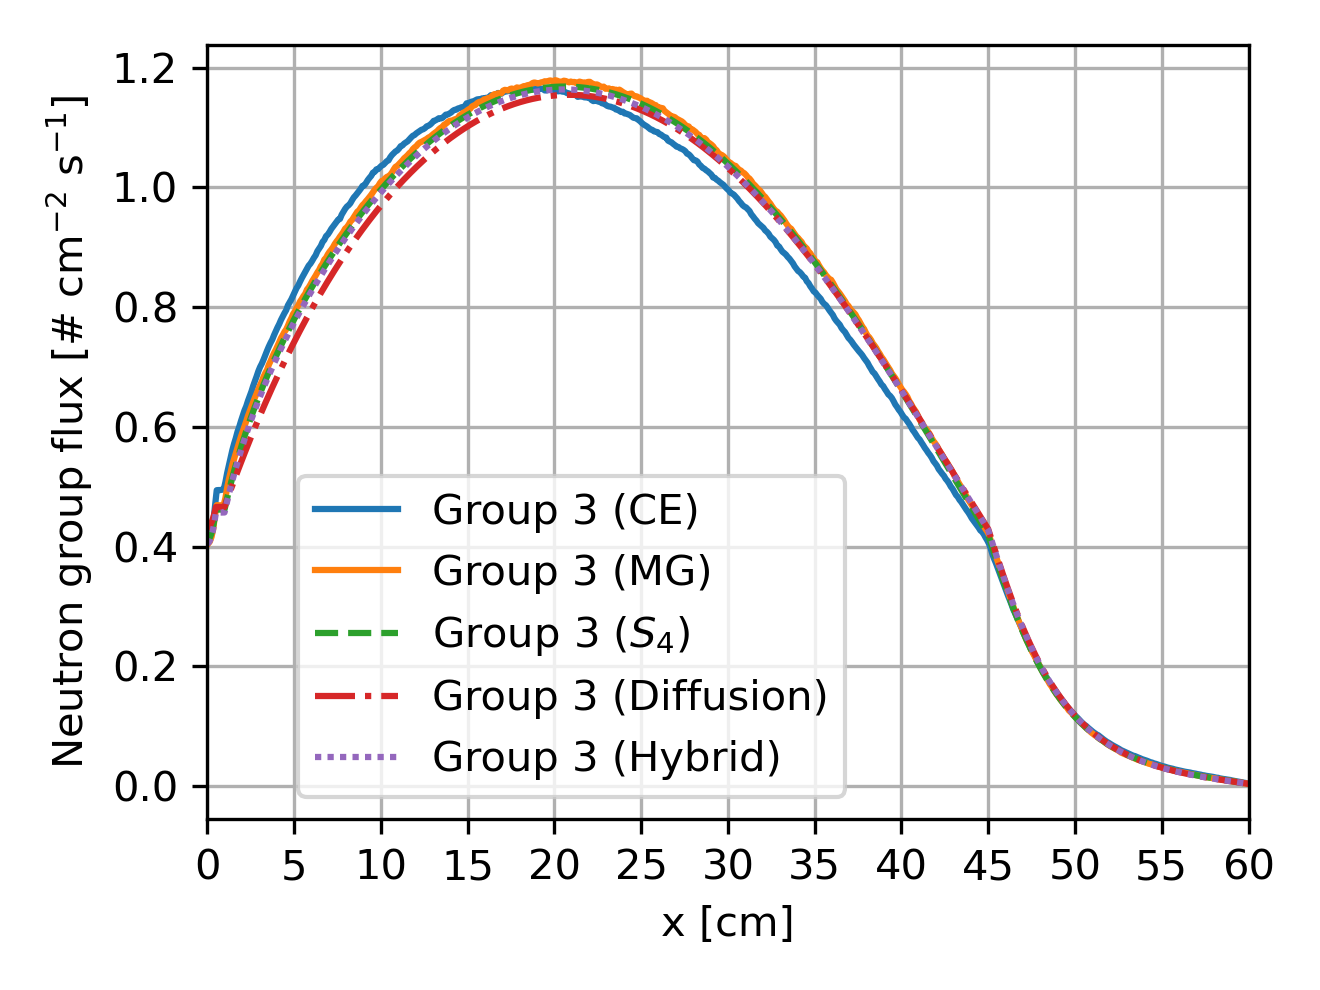
\includegraphics[width=\textwidth]{../images/case-3b-group-3-flux}
        \label{fig:c3bg3}
      \end{subfigure}
      \begin{subfigure}[t]{.45\textwidth}
        \centering
        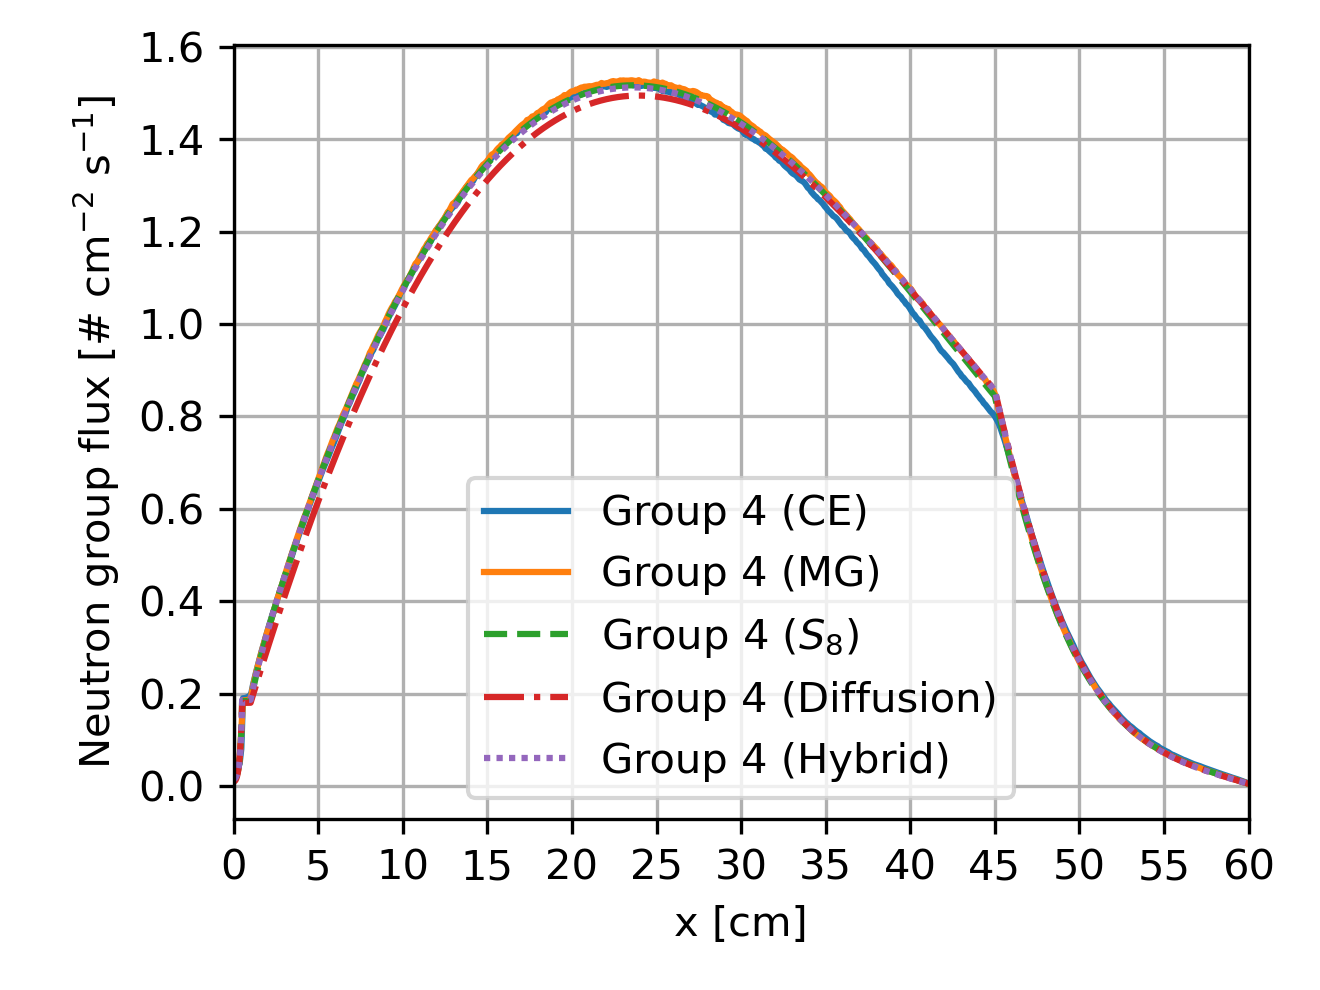
\includegraphics[width=\textwidth]{../images/case-3b-group-4-flux}
        \label{fig:c3bg4}
      \end{subfigure}
      \caption{Neutron group flux distributions for Case 3b.}
      \label{fig:c3bflux}
    \end{figure}
    \column{4cm}
    \begin{itemize}
      \item The OpenMC-CE (blue) and neutron diffusion (red) flux solutions deviate from the rest
      \item Discrepancy with the OpenMC-CE solution is likely due to neutron energy group
        discretization
    \end{itemize}
  \end{columns}
\end{frame}

\begin{frame}
  \frametitle{Hybrid $S_N$-Diffusion Method: Preliminary Results}
  \begin{figure}
    \centering
    \begin{subfigure}[t]{.34\textwidth}
      \centering
      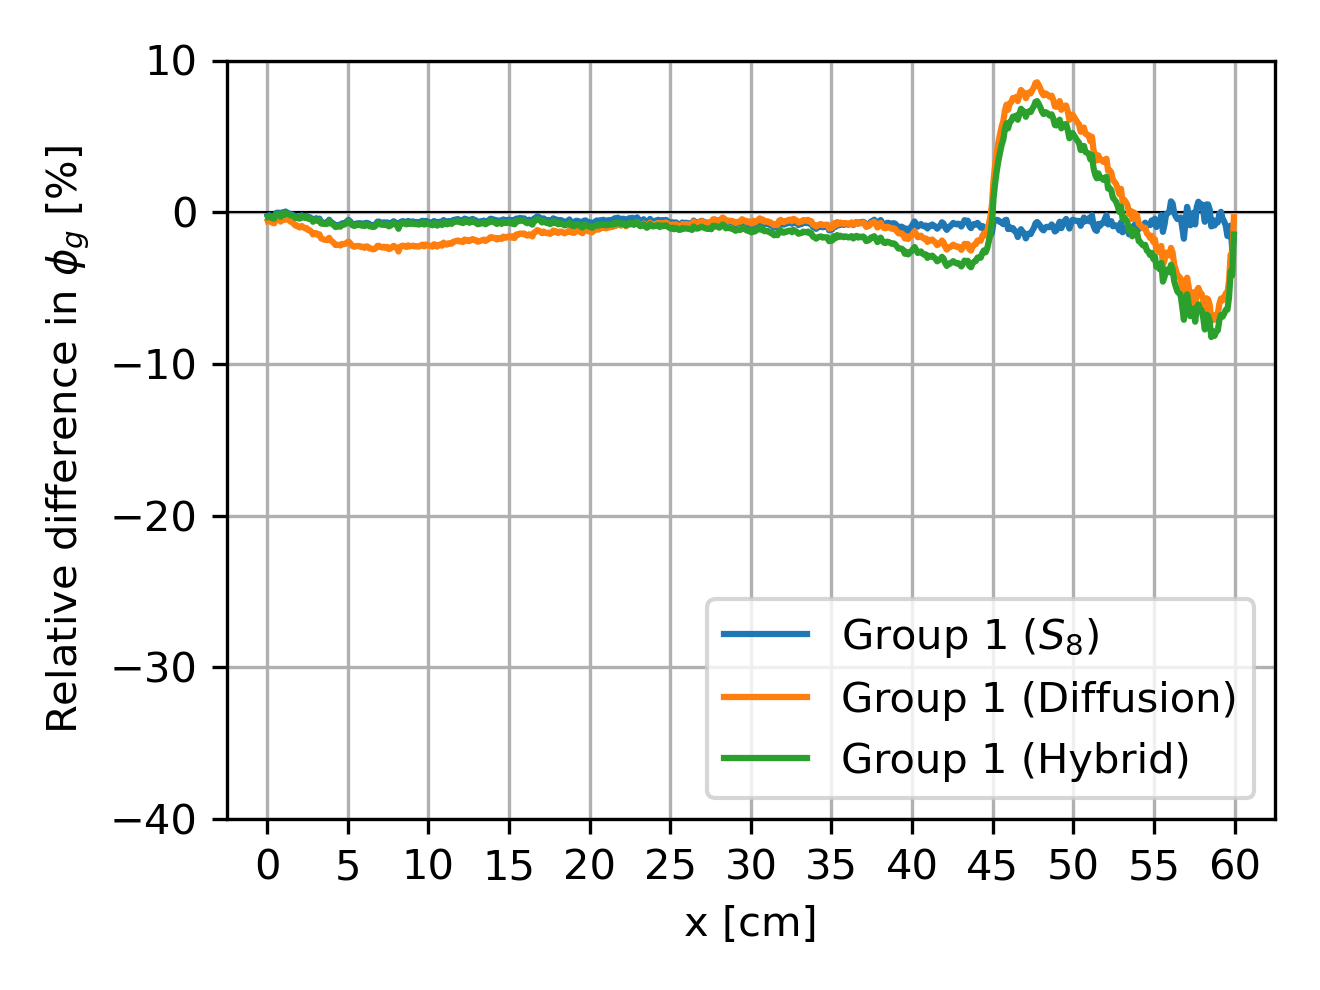
\includegraphics[width=\textwidth]{../images/case-3b-group-1-flux-error}
      \label{fig:c3bg1e}
    \end{subfigure}
    \begin{subfigure}[t]{.34\textwidth}
      \centering
      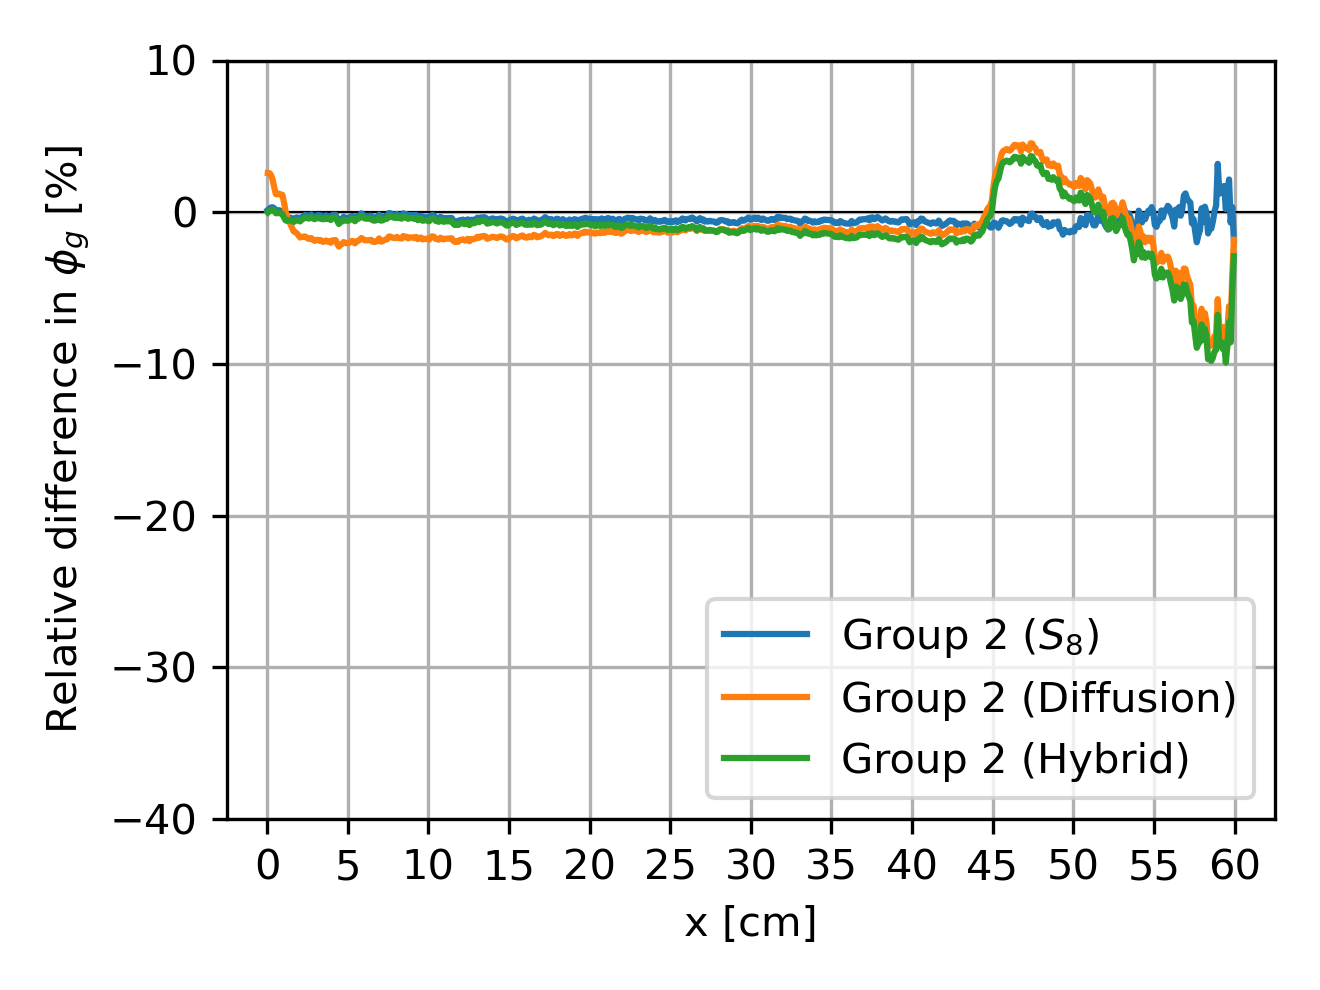
\includegraphics[width=\textwidth]{../images/case-3b-group-2-flux-error}
      \label{fig:c3bg2e}
    \end{subfigure}
    \begin{subfigure}[t]{.34\textwidth}
      \centering
      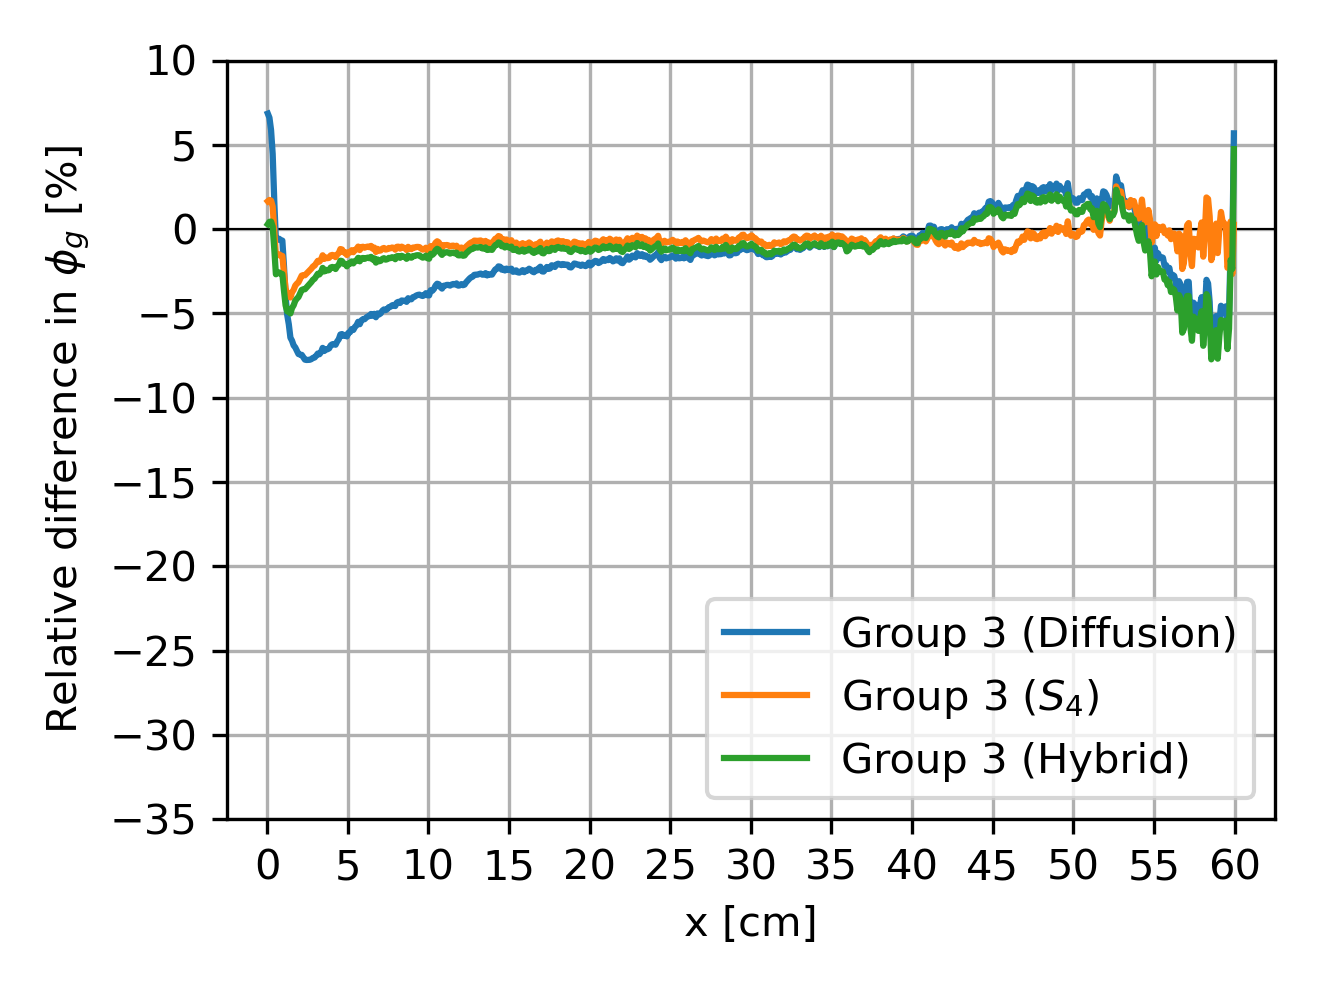
\includegraphics[width=\textwidth]{../images/case-3b-group-3-flux-error}
      \label{fig:c3bg3e}
    \end{subfigure}
    \begin{subfigure}[t]{.34\textwidth}
      \centering
      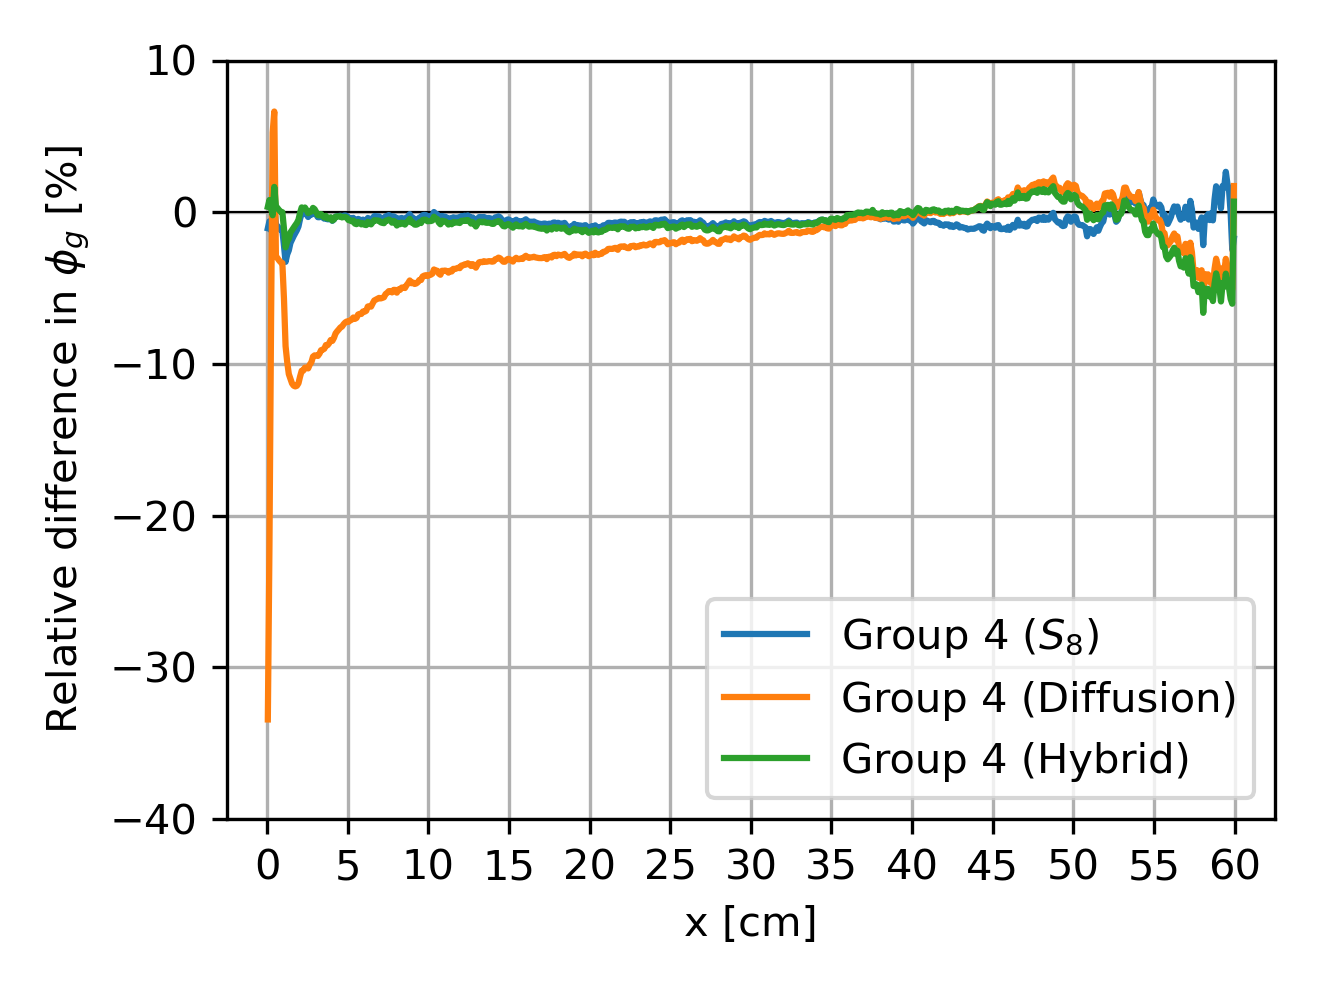
\includegraphics[width=\textwidth]{../images/case-3b-group-4-flux-error}
      \label{fig:c3bg4e}
    \end{subfigure}
    \caption{Relative differences of the neutron group flux distributions for Case 3b with respect
    to OpenMC-MG.}
    \label{fig:c3bfluxe}
  \end{figure}
\end{frame}

\begin{frame}
  \frametitle{Hybrid $S_N$-Diffusion Method: Preliminary Results}
  \begin{figure}[htb!]
    \centering
    \begin{subfigure}[t]{.35\textwidth}
      \centering
      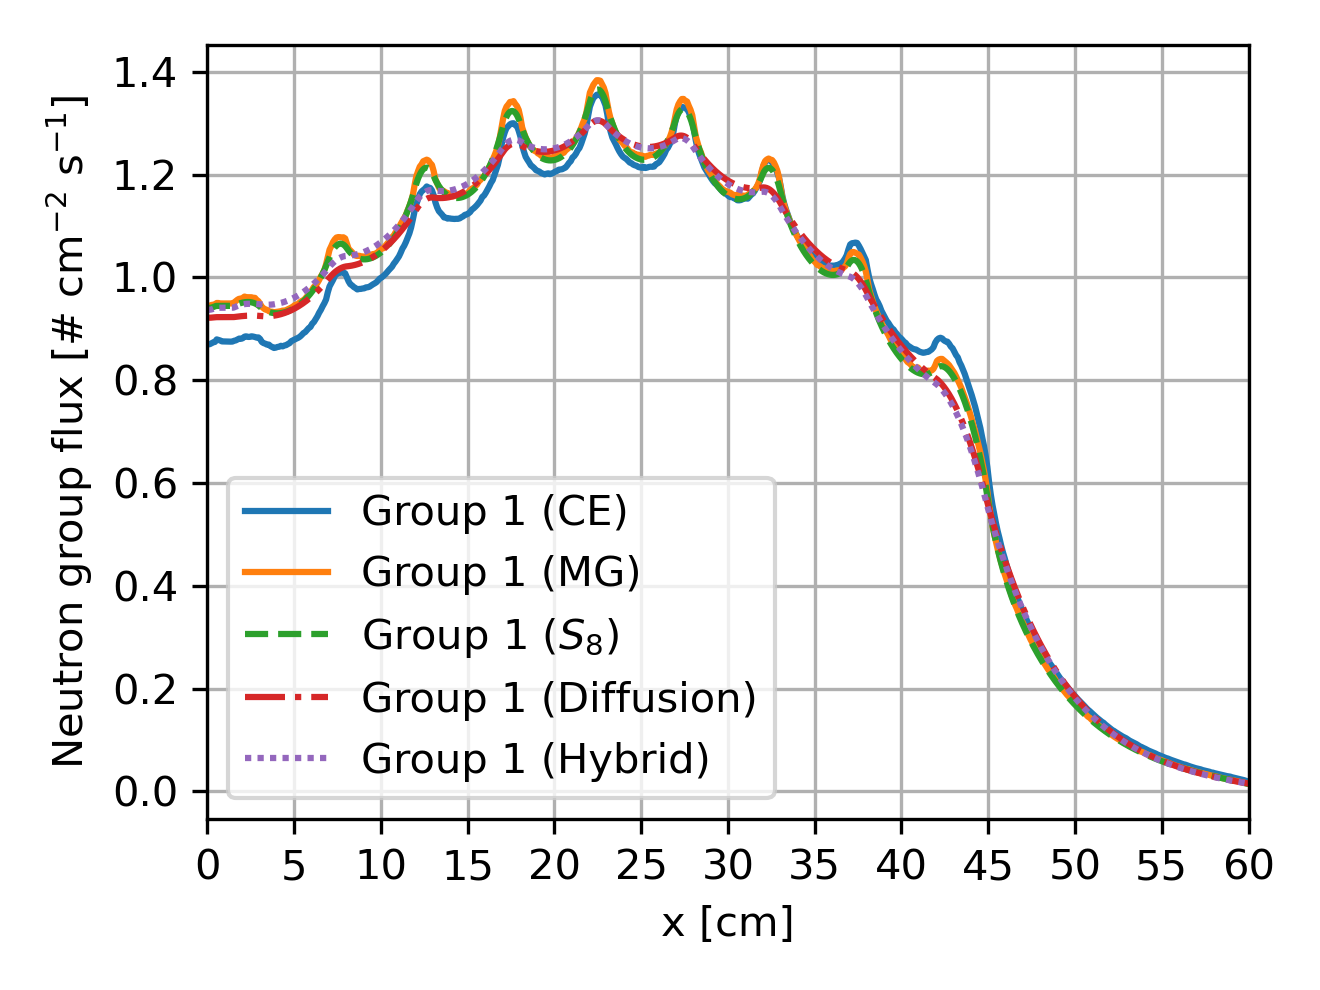
\includegraphics[width=\textwidth]{../images/case-5a-group-1-flux}
      \label{fig:c5ag1}
    \end{subfigure}
    \begin{subfigure}[t]{.35\textwidth}
      \centering
      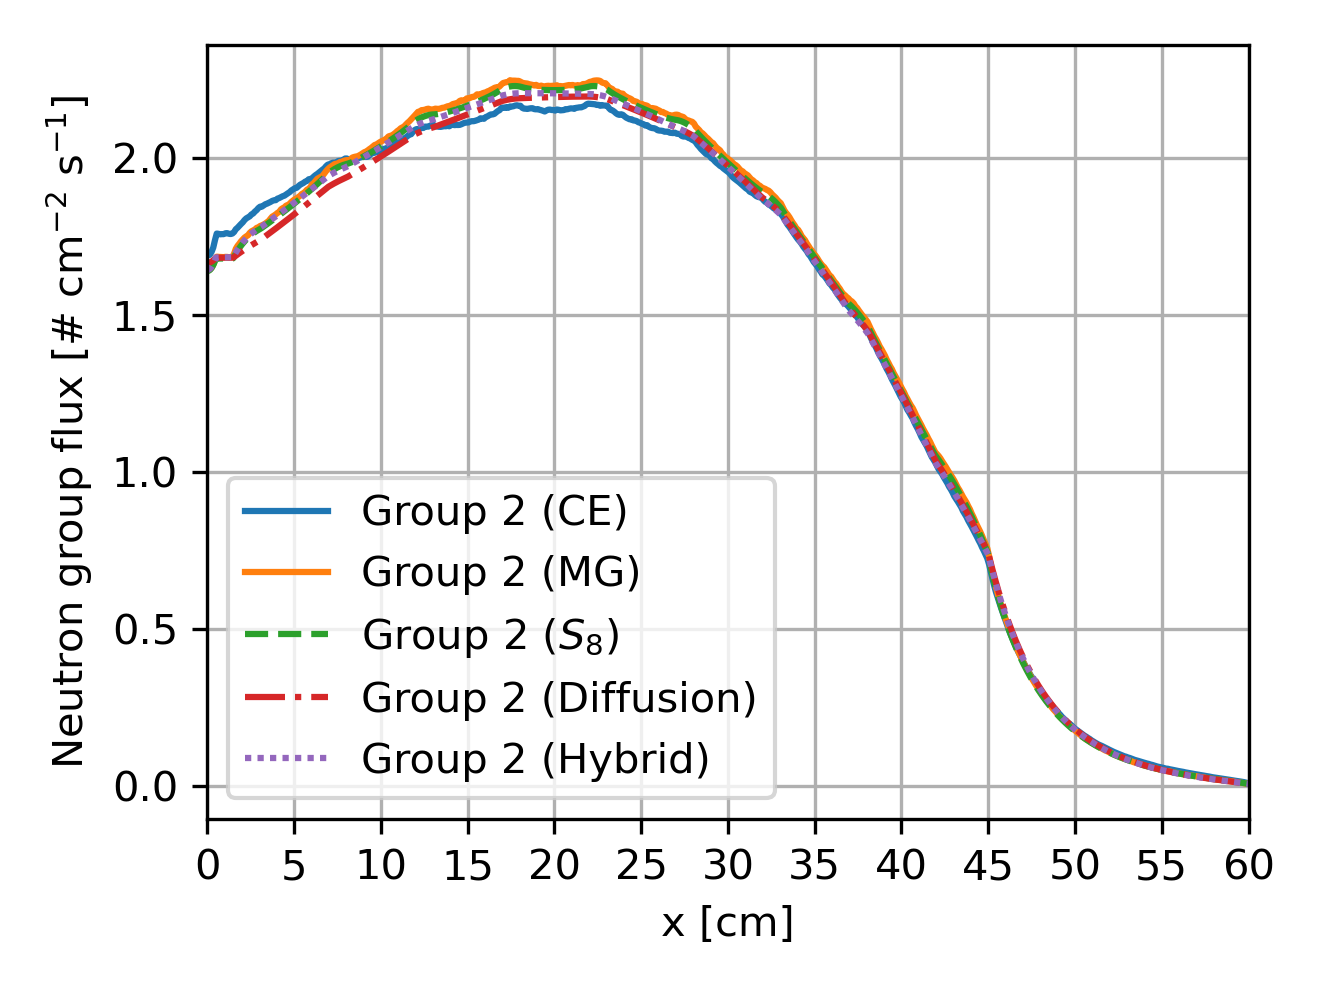
\includegraphics[width=\textwidth]{../images/case-5a-group-2-flux}
      \label{fig:c5ag2}
    \end{subfigure}
    \begin{subfigure}[t]{.35\textwidth}
      \centering
      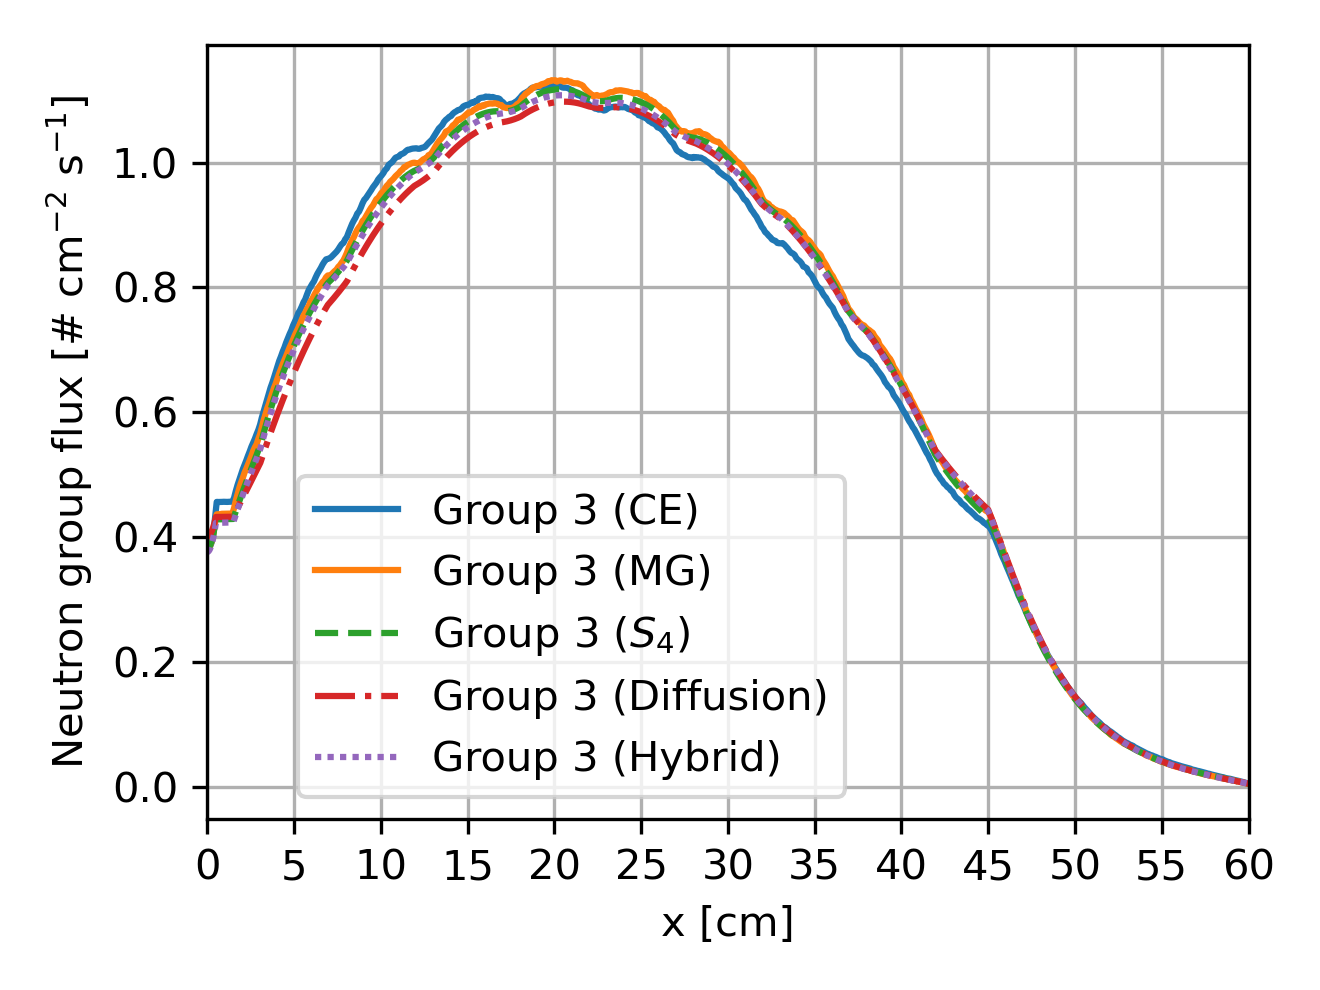
\includegraphics[width=\textwidth]{../images/case-5a-group-3-flux}
      \label{fig:c5ag3}
    \end{subfigure}
    \begin{subfigure}[t]{.35\textwidth}
      \centering
      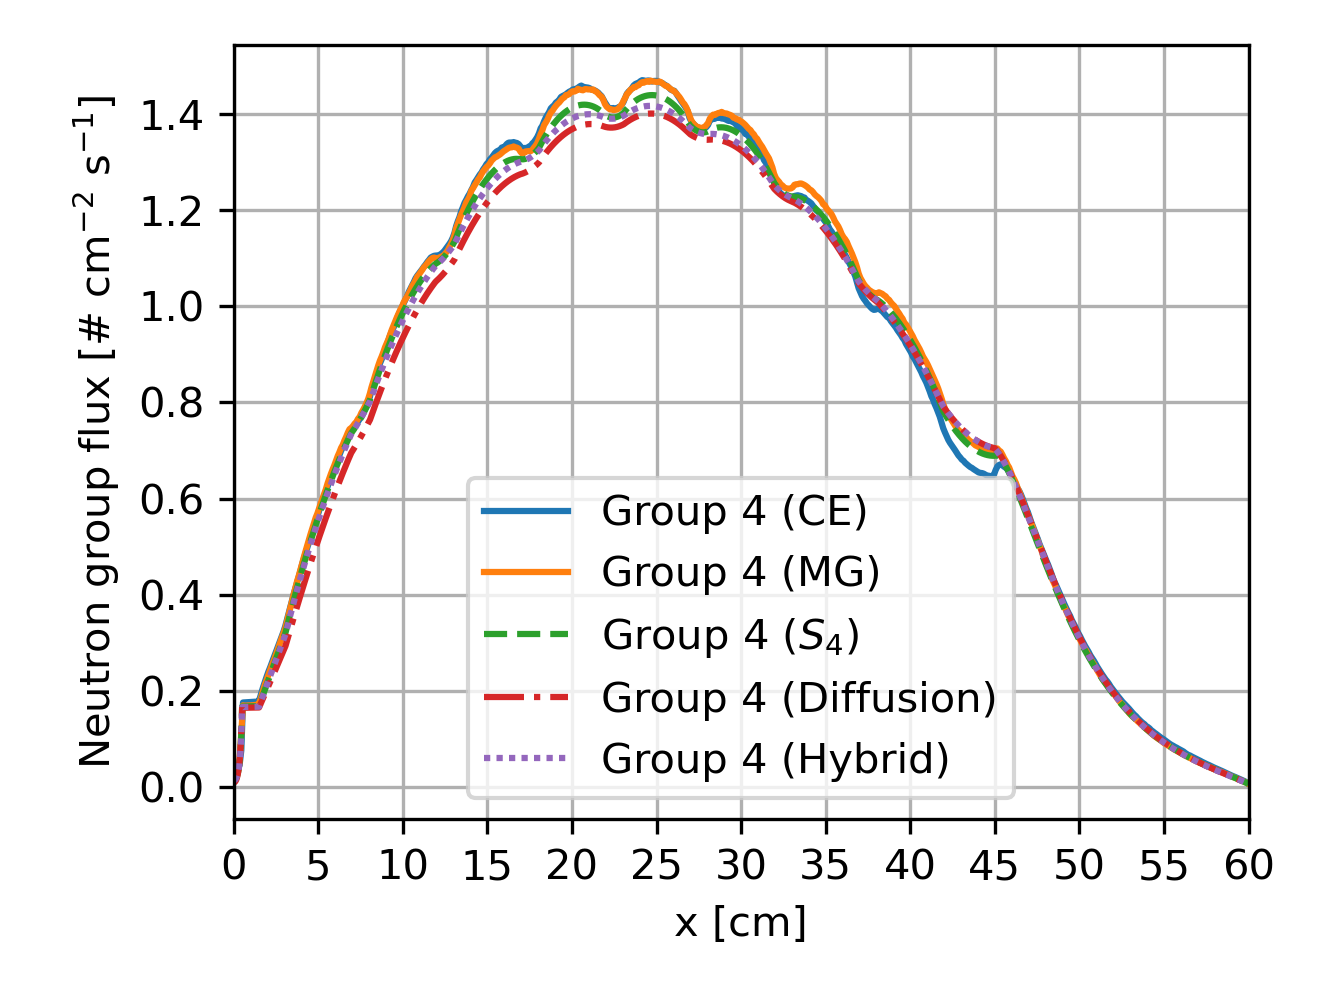
\includegraphics[width=\textwidth]{../images/case-5a-group-4-flux}
      \label{fig:c5ag4}
    \end{subfigure}
    \caption{Neutron group flux distributions for Case 5a.}
    \label{fig:c5aflux}
  \end{figure}
\end{frame}

\begin{frame}
  \frametitle{Hybrid $S_N$-Diffusion Method: Preliminary Results}
  \begin{figure}[htb!]
    \centering
    \begin{subfigure}[t]{.34\textwidth}
      \centering
      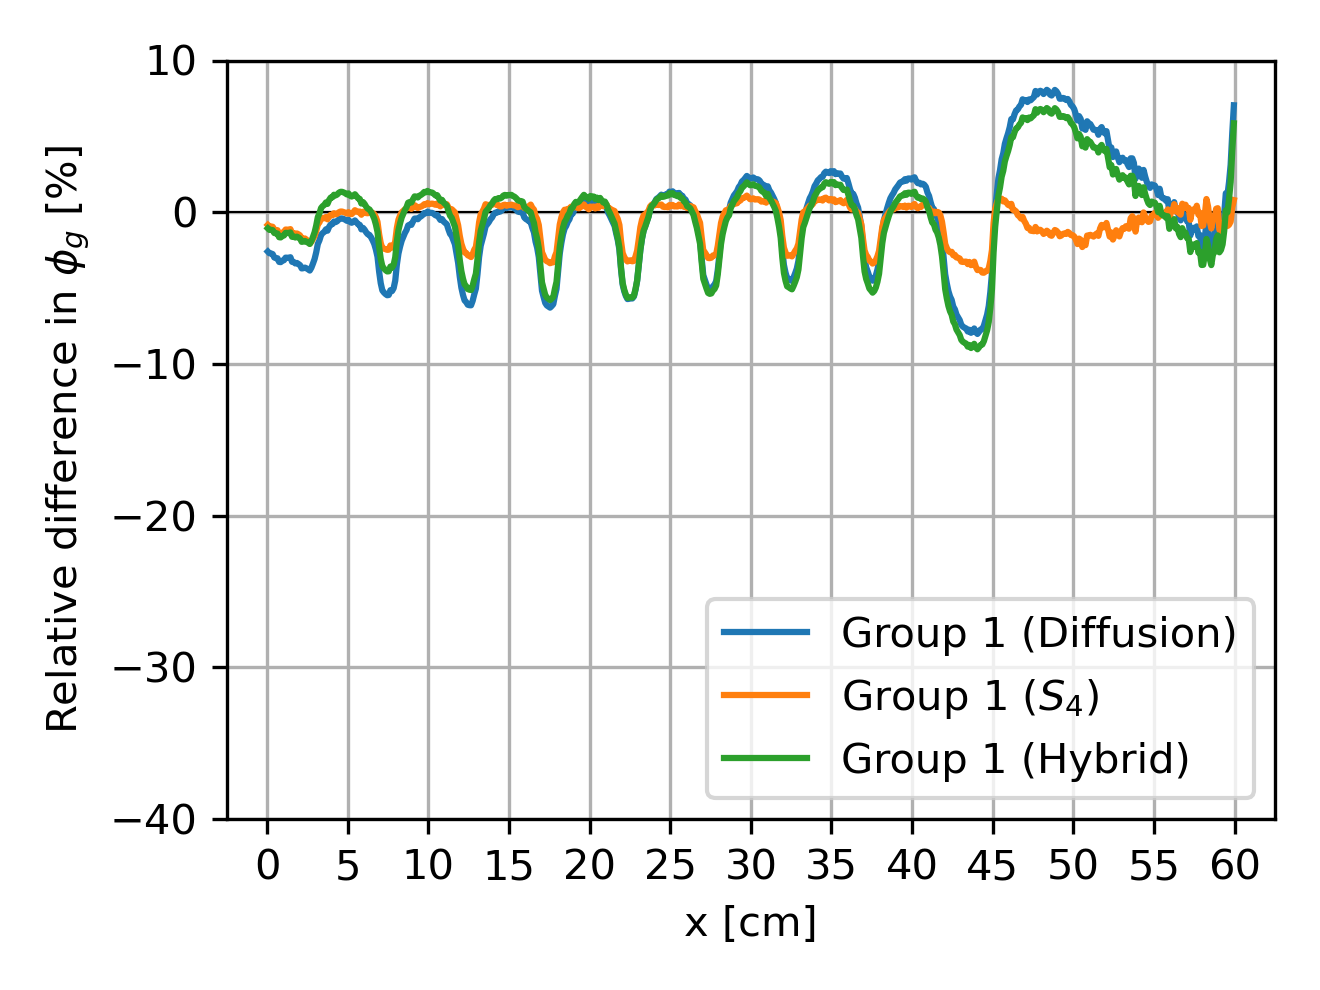
\includegraphics[width=\textwidth]{../images/case-5a-group-1-flux-error}
      \label{fig:c5ag1e}
    \end{subfigure}
    \begin{subfigure}[t]{.34\textwidth}
      \centering
      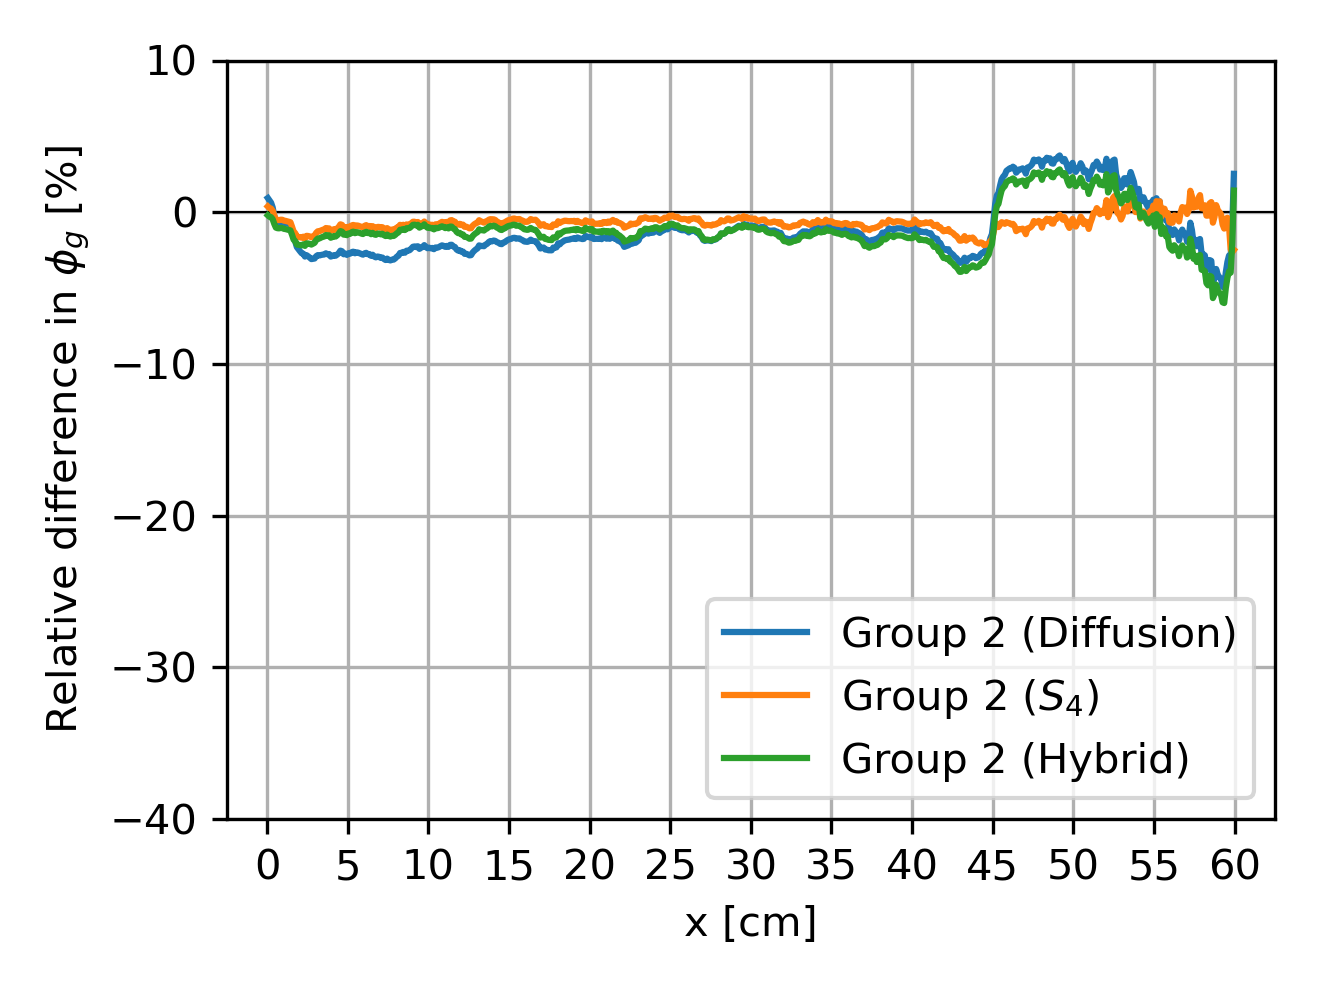
\includegraphics[width=\textwidth]{../images/case-5a-group-2-flux-error}
      \label{fig:c5ag2e}
    \end{subfigure}
    \begin{subfigure}[t]{.34\textwidth}
      \centering
      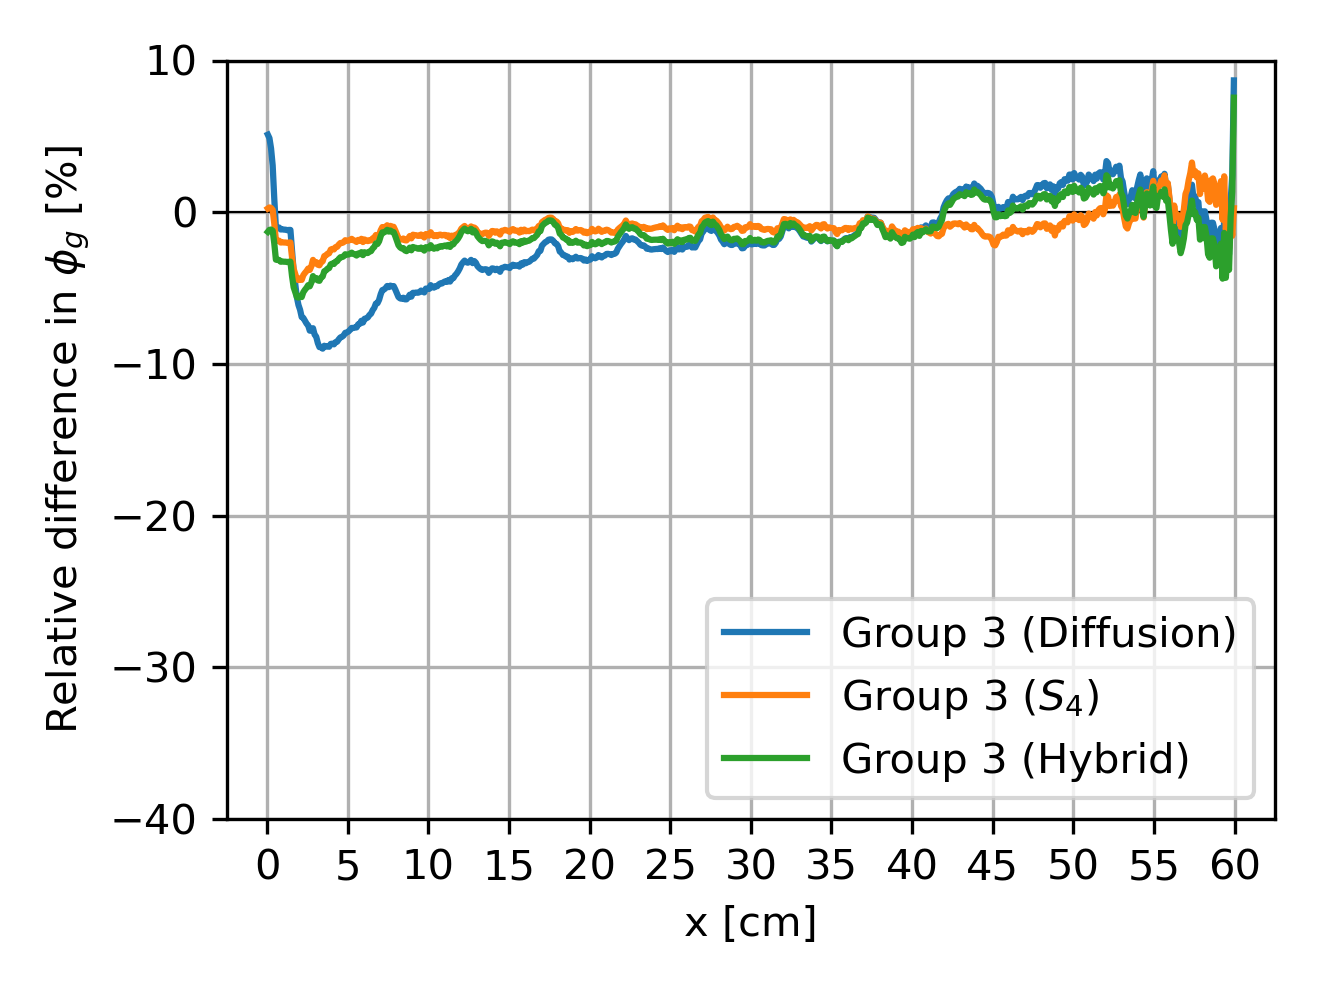
\includegraphics[width=\textwidth]{../images/case-5a-group-3-flux-error}
      \label{fig:c5ag3e}
    \end{subfigure}
    \begin{subfigure}[t]{.34\textwidth}
      \centering
      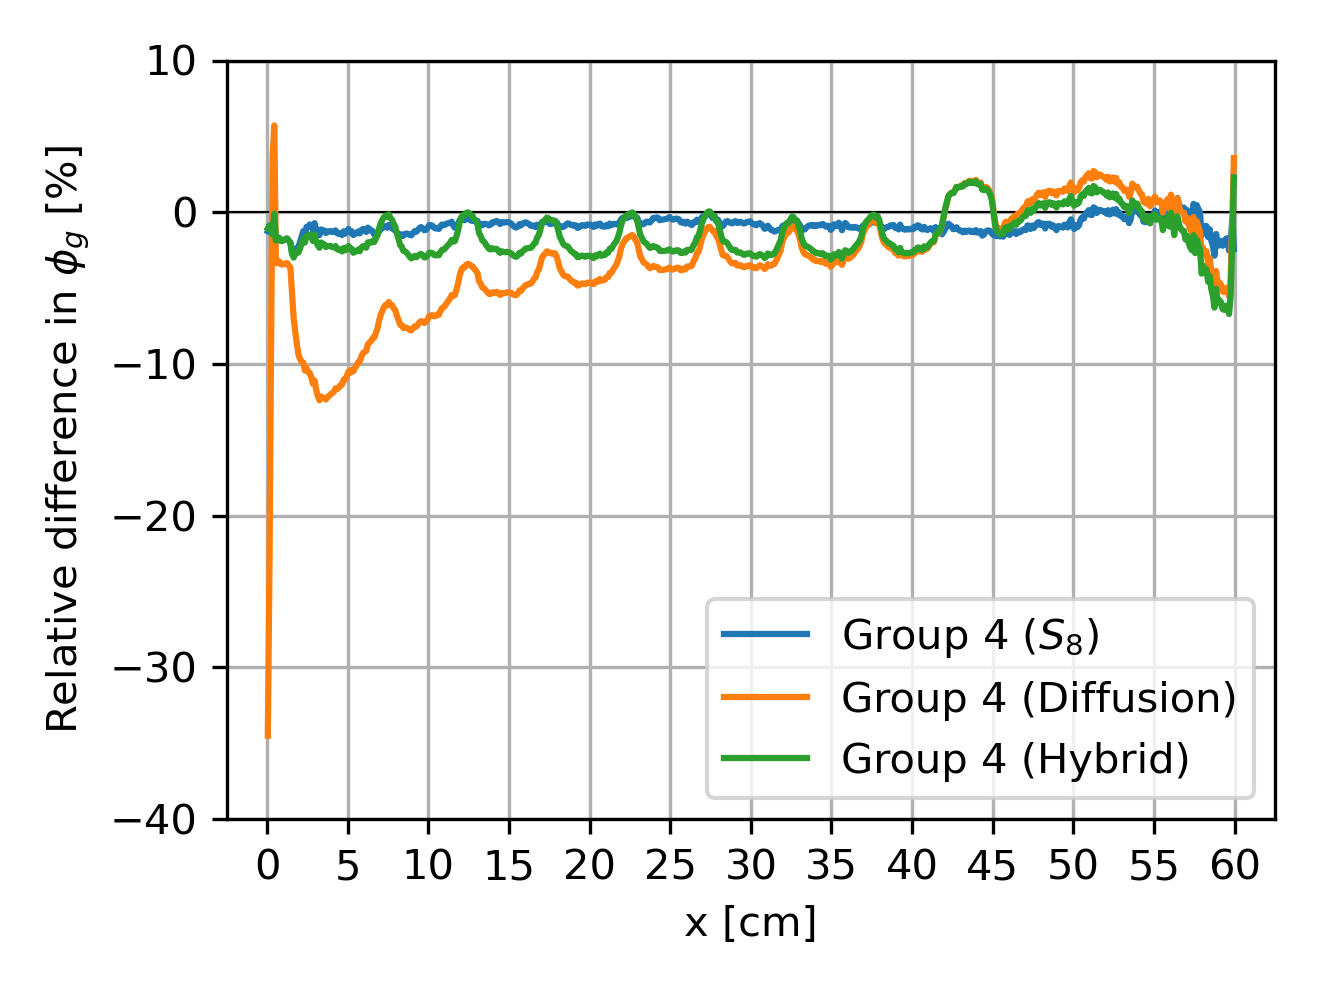
\includegraphics[width=\textwidth]{../images/case-5a-group-4-flux-error}
      \label{fig:c5ag4e}
    \end{subfigure}
    \caption{Relative differences of the neutron group flux distributions for Case 5a with respect
    to OpenMC-MG.}
    \label{fig:c5afluxe}
  \end{figure}
\end{frame}

%\begin{frame}
%  \frametitle{Hybrid $S_N$-Diffusion Method: Preliminary Results}
%  \begin{table}
%    \centering
%    \footnotesize
%    \caption{Normalized flux error $\varepsilon$ for Case 3b with respect to OpenMC-MG.}
%    \begin{tabular}{c S S S S}
%      \toprule
%      {\multirow{2}{*}{\textbf{Method}}} &
%      \multicolumn{4}{c}{\textbf{Normalized flux error,} $\bm{\varepsilon_g}$} \\
%      \cmidrule{2-5}
%      & {\textbf{Group 1}} & {\textbf{Group 2}} & {\textbf{Group 3}} &
%      {\textbf{Group 4}} \\
%      \midrule
%      $S_8$     & 0.0066 & 0.0048 & 0.0058 & 0.0067 \\
%      Diffusion & 0.0144 & 0.0147 & 0.0258 & 0.0267 \\
%      Hybrid    & 0.0122 & 0.0099 & 0.0087 & 0.0084 \\
%      \bottomrule
%    \end{tabular}
%    \label{table:c3berror}
%  \end{table}
%  \begin{table}
%    \centering
%    \footnotesize
%    \caption{Normalized flux error $\varepsilon$ for Case 5a with respect to OpenMC-MG.}
%    \begin{tabular}{c S S S S}
%      \toprule
%      {\multirow{2}{*}{\textbf{Method}}} &
%      \multicolumn{4}{c}{\textbf{Normalized flux error,} $\bm{\varepsilon_g}$} \\
%      \cmidrule{2-5}
%      & {\textbf{Group 1}} & {\textbf{Group 2}} & {\textbf{Group 3}} &
%      {\textbf{Group 4}} \\
%      \midrule
%      $S_8$     & 0.0078 & 0.0074 & 0.0083 & 0.0085 \\
%      Diffusion & 0.0305 & 0.0202 & 0.0313 & 0.0406 \\
%      Hybrid    & 0.0290 & 0.0147 & 0.0143 & 0.0216 \\
%      \bottomrule
%    \end{tabular}
%    \label{table:c5aerror}
%  \end{table}
%\end{frame}

\begin{frame}
  \frametitle{Hybrid $S_N$-Diffusion Method: Preliminary Results}
  \begin{figure}
    \centering
    \begin{subfigure}[t]{.35\textwidth}
      \centering
      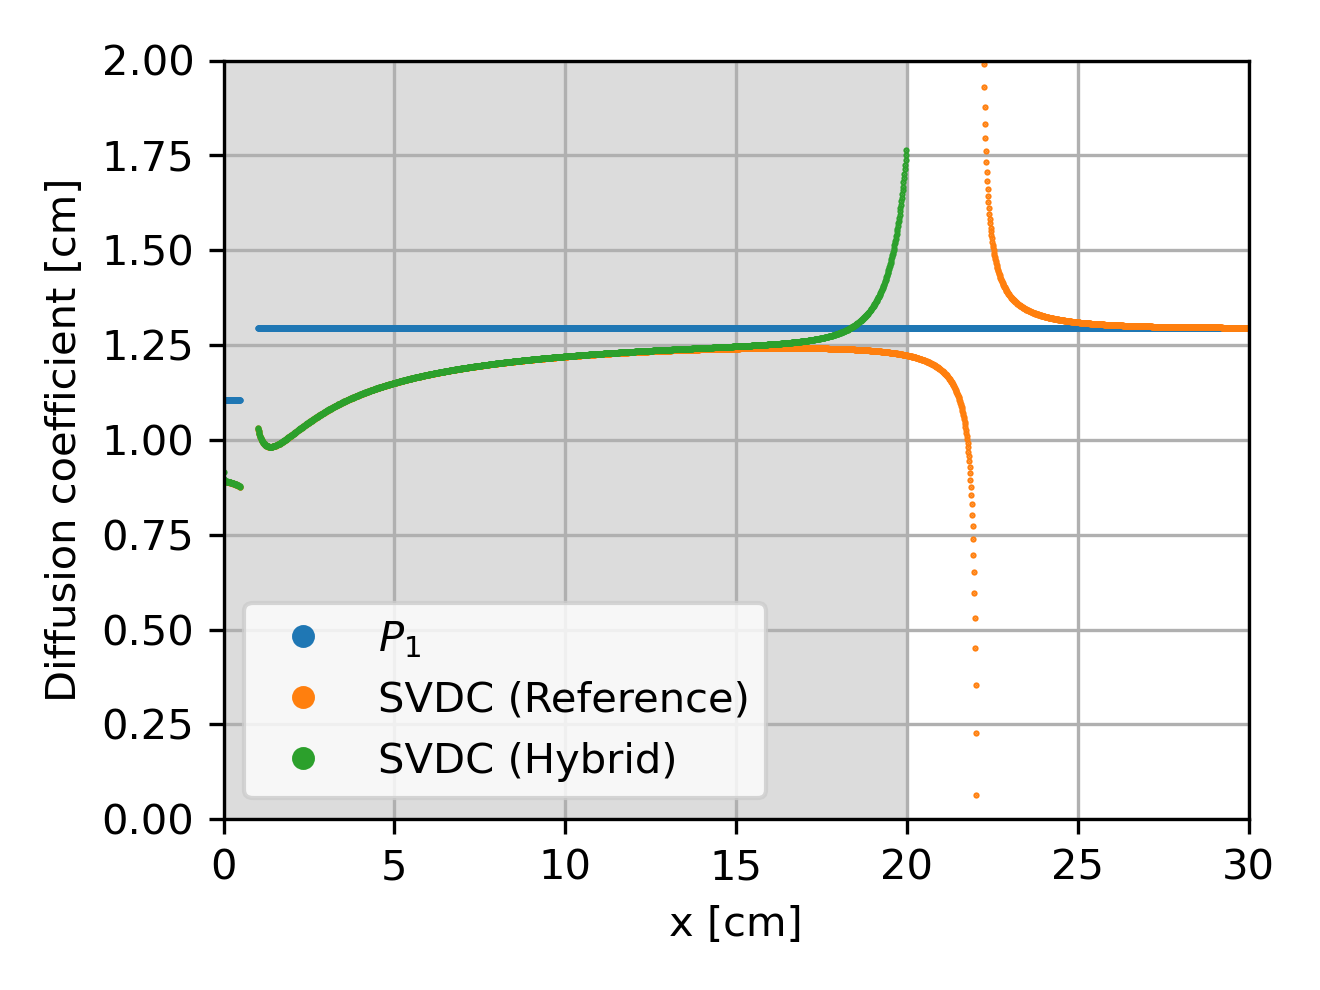
\includegraphics[width=\textwidth]{images/case-3b-group-1-diffcoef}
      \label{fig:c3bg1dc}
    \end{subfigure}
    \begin{subfigure}[t]{.35\textwidth}
      \centering
      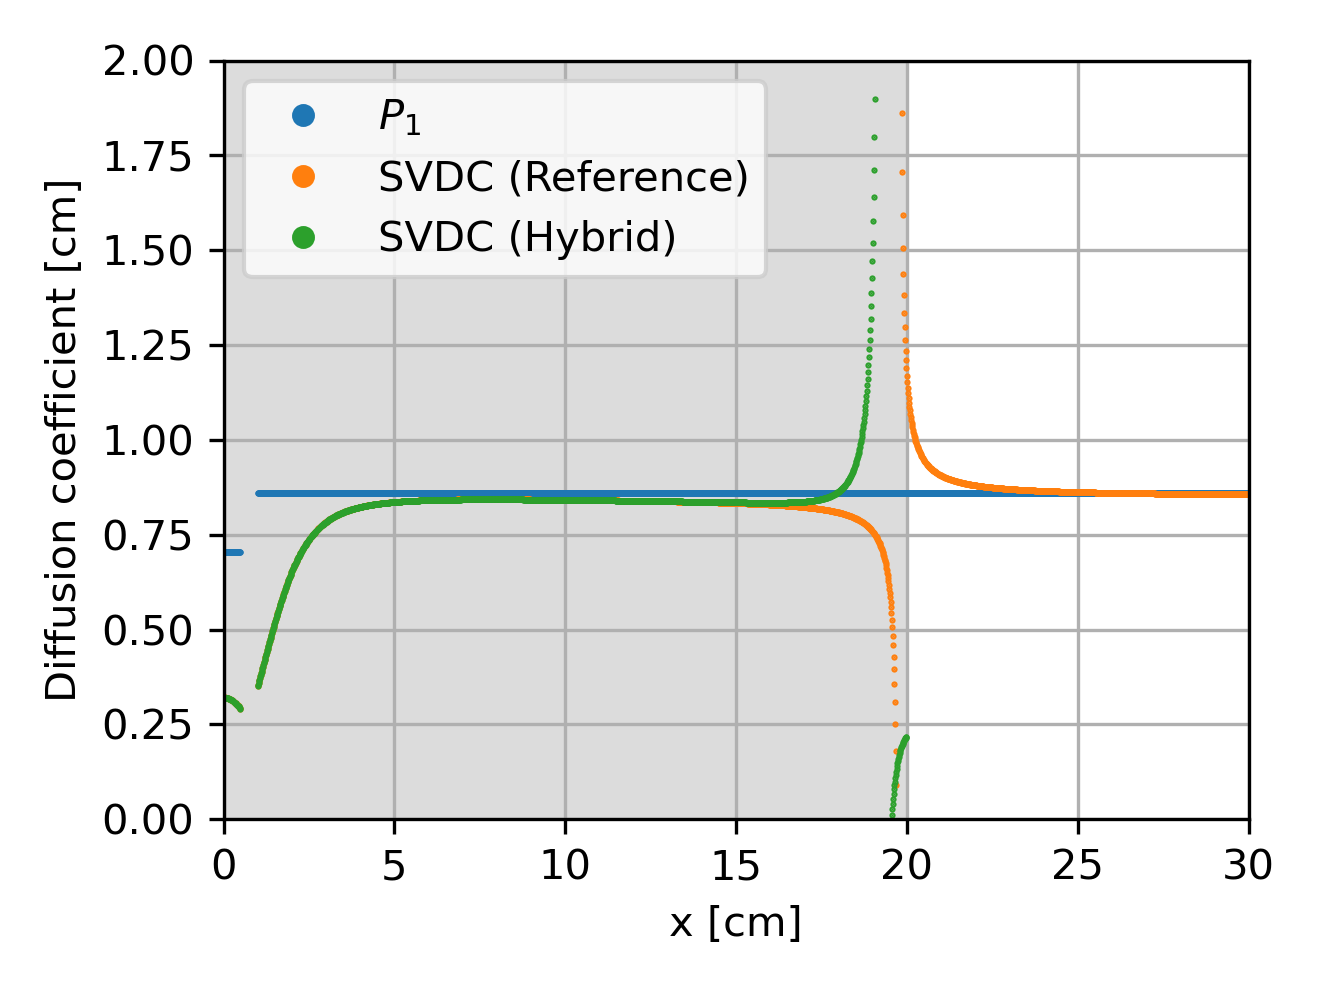
\includegraphics[width=\textwidth]{images/case-3b-group-2-diffcoef}
      \label{fig:c3bg2dc}
    \end{subfigure}
    \begin{subfigure}[t]{.35\textwidth}
      \centering
      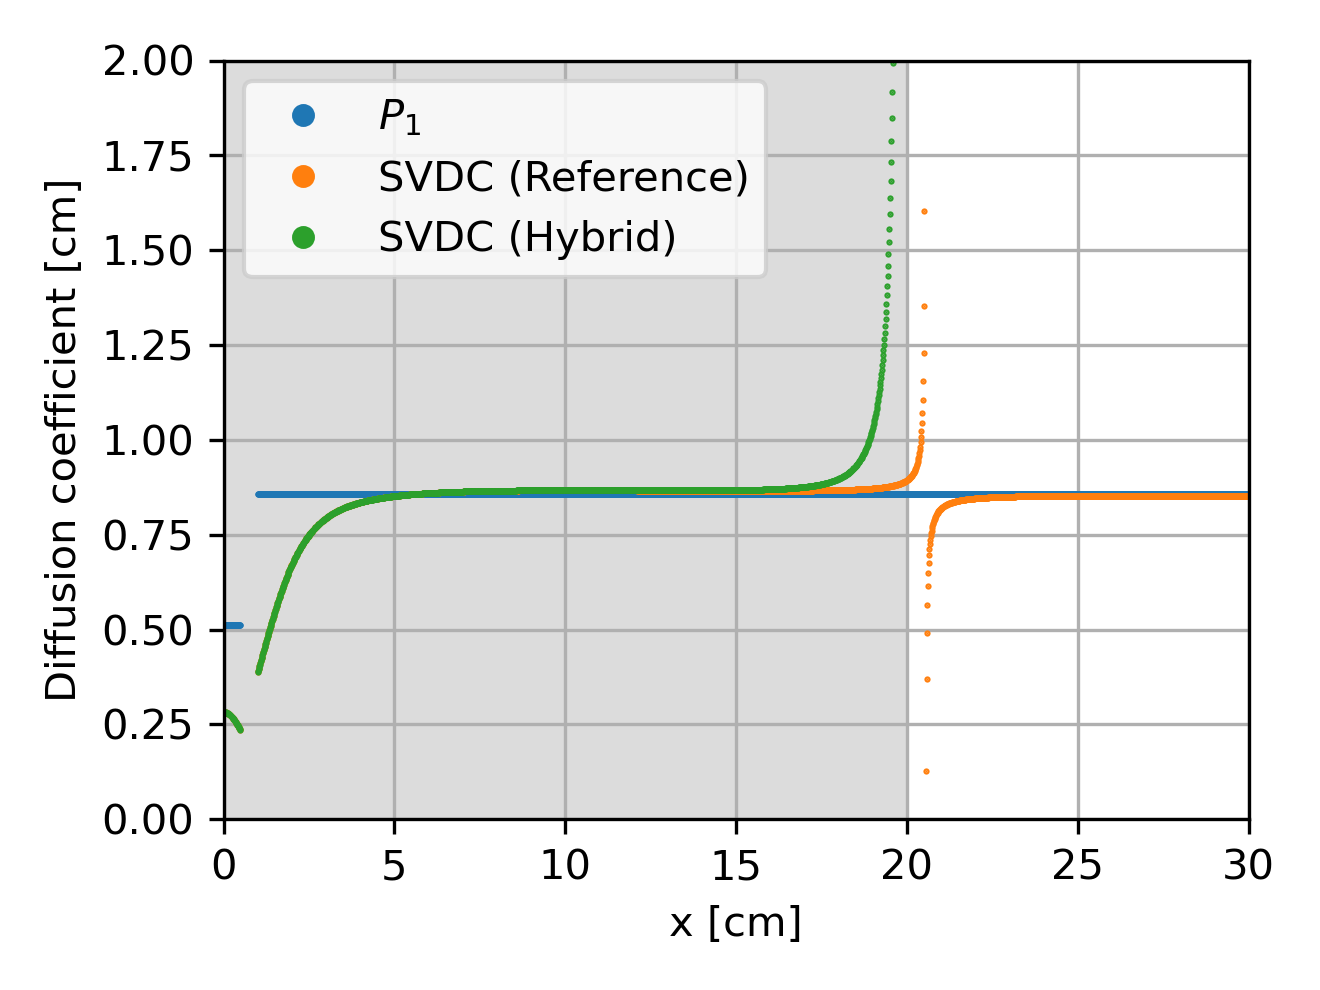
\includegraphics[width=\textwidth]{images/case-3b-group-3-diffcoef}
      \label{fig:c3bg3dc}
    \end{subfigure}
    \begin{subfigure}[t]{.35\textwidth}
      \centering
      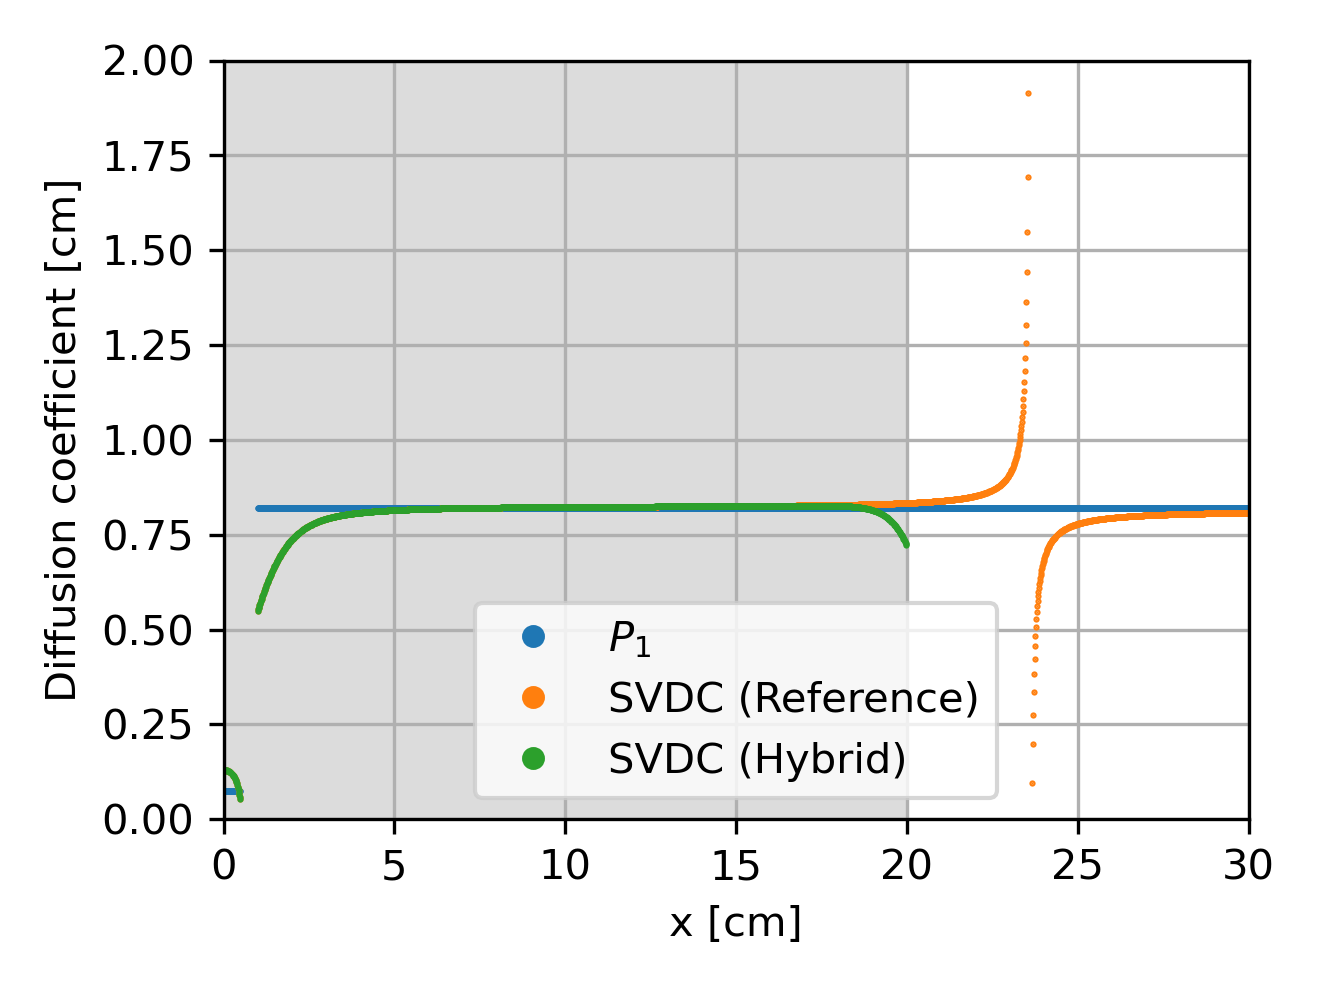
\includegraphics[width=\textwidth]{images/case-3b-group-4-diffcoef}
      \label{fig:c3bg4dc}
    \end{subfigure}
    \caption{Diffusion coefficients for Case 3b between $x=0$ cm and $x=30$ cm.}
    \label{fig:c3bdiffcoef}
  \end{figure}
\end{frame}

\begin{frame}
  \frametitle{Hybrid $S_N$-Diffusion Method: Preliminary Results}
  \begin{figure}
    \centering
    \begin{subfigure}[t]{.35\textwidth}
      \centering
      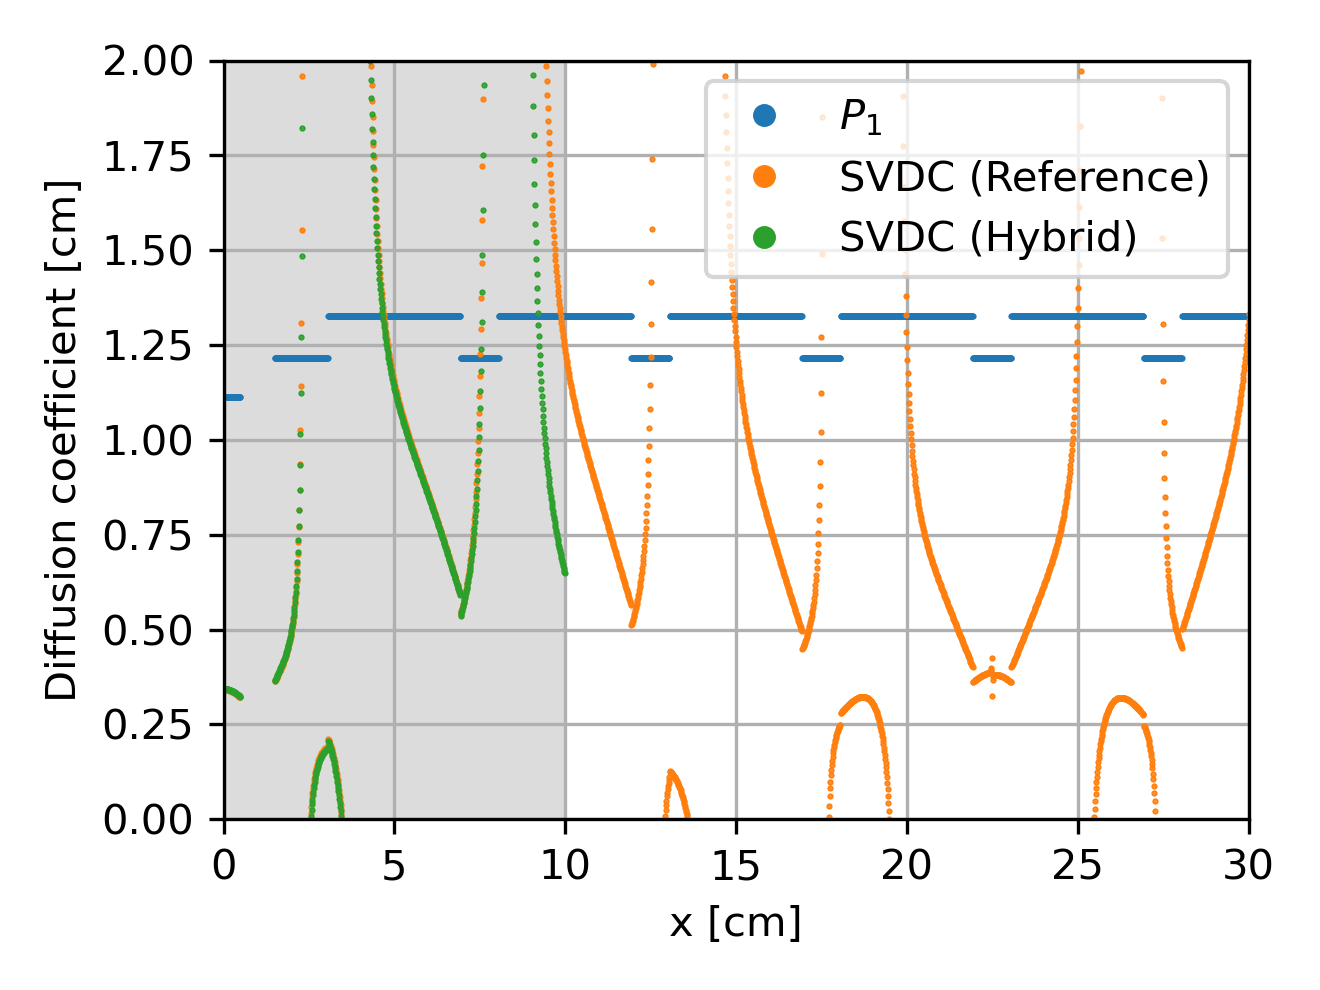
\includegraphics[width=\textwidth]{images/case-5a-group-1-diffcoef}
      \label{fig:c5ag1dc}
    \end{subfigure}
    \begin{subfigure}[t]{.35\textwidth}
      \centering
      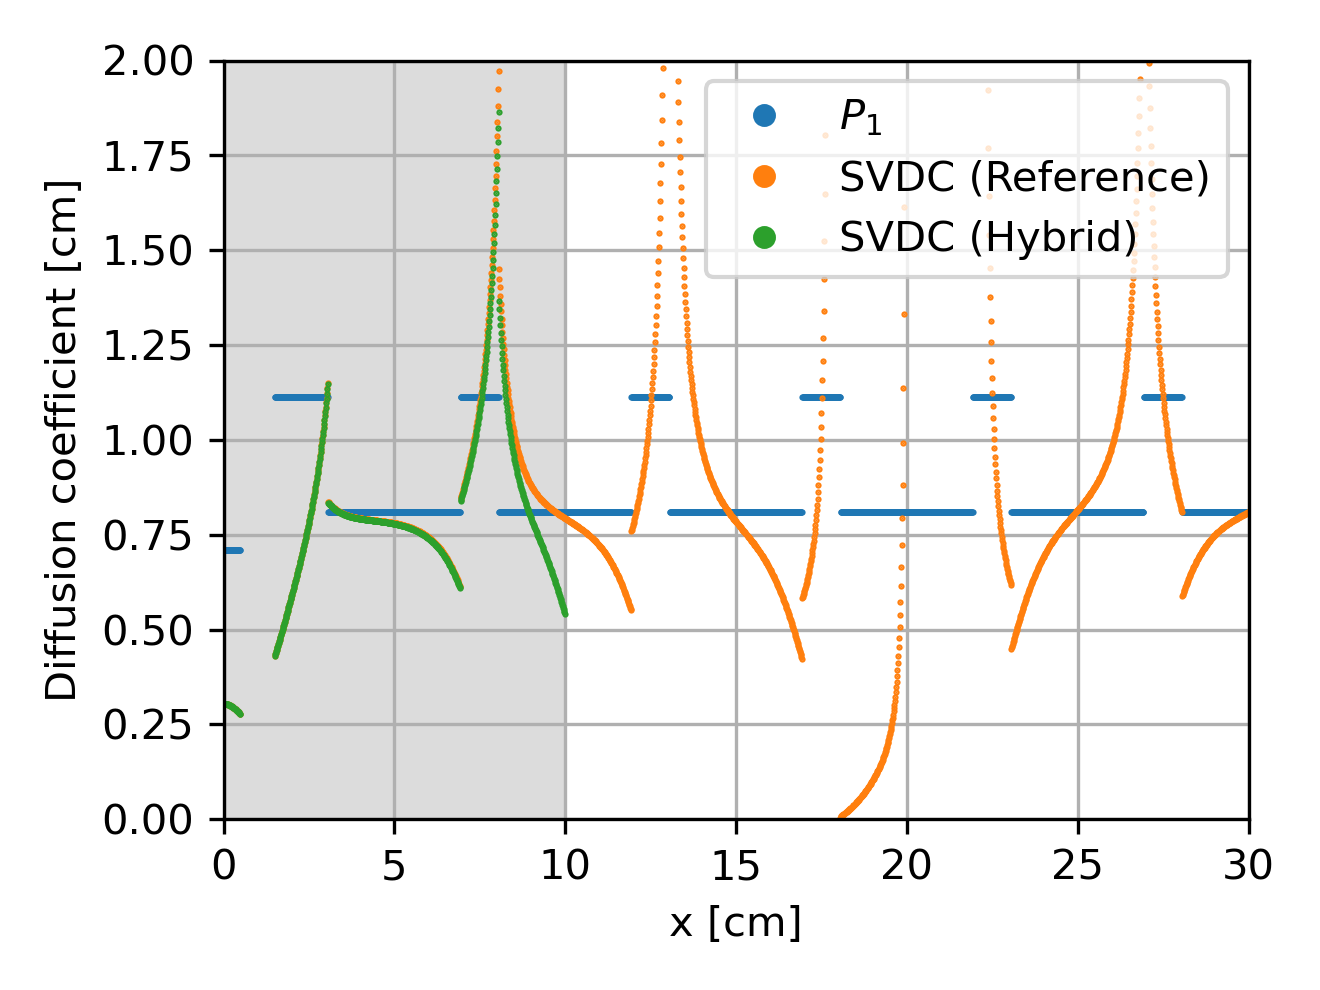
\includegraphics[width=\textwidth]{images/case-5a-group-2-diffcoef}
      \label{fig:c5ag2dc}
    \end{subfigure}
    \begin{subfigure}[t]{.35\textwidth}
      \centering
      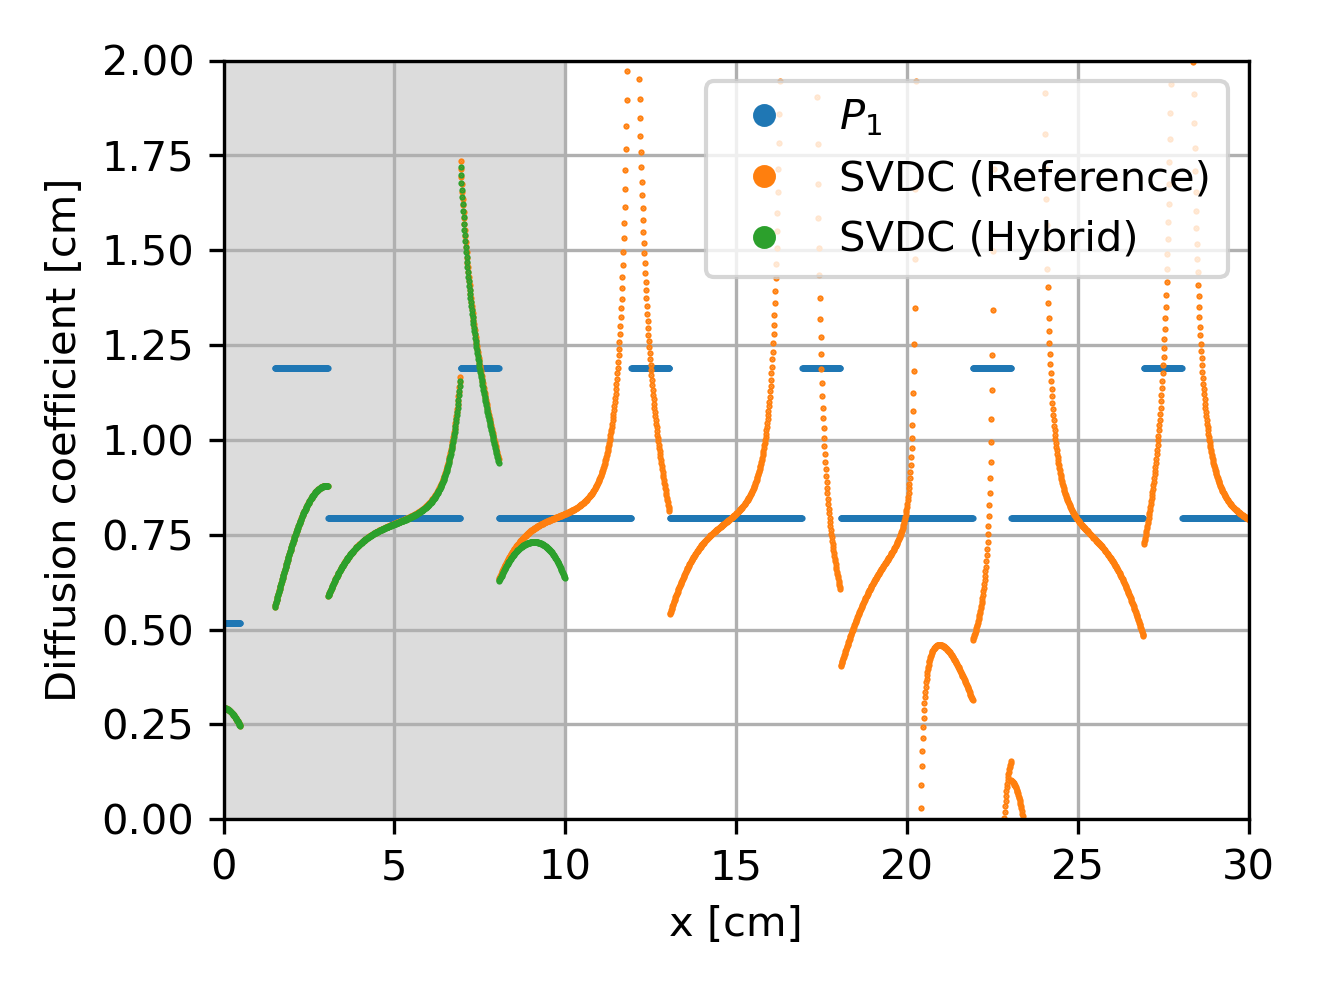
\includegraphics[width=\textwidth]{images/case-5a-group-3-diffcoef}
      \label{fig:c5ag3dc}
    \end{subfigure}
    \begin{subfigure}[t]{.35\textwidth}
      \centering
      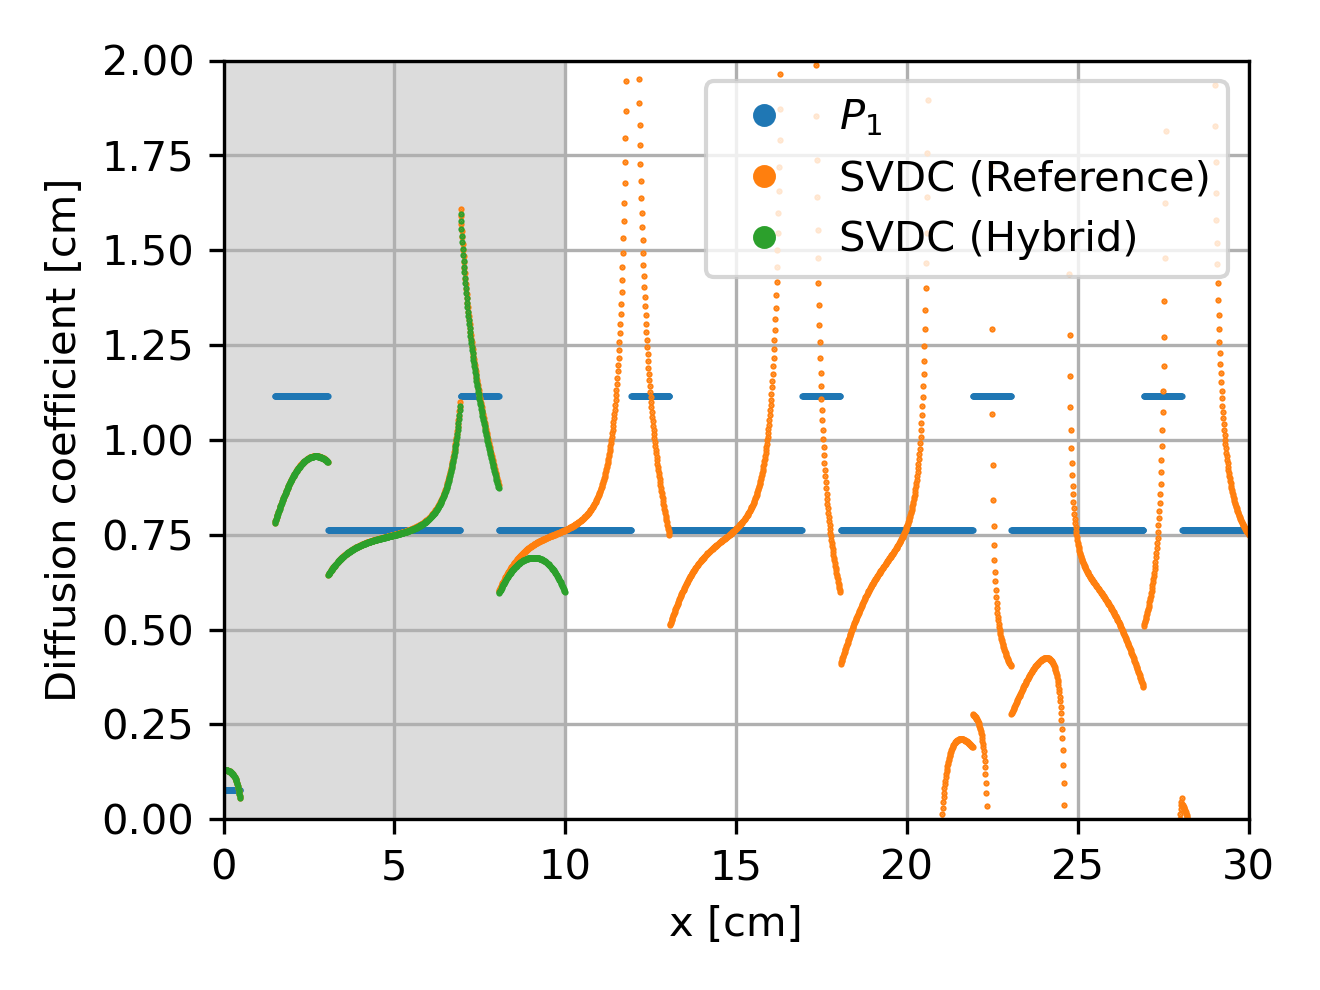
\includegraphics[width=\textwidth]{images/case-5a-group-4-diffcoef}
      \label{fig:c5ag4dc}
    \end{subfigure}
    \caption{Diffusion coefficients for Case 5a between $x=0$ cm and $x=30$ cm.}
    \label{fig:c5adiffcoef}
  \end{figure}
\end{frame}

\begin{frame}
  \frametitle{Hybrid $S_N$-Diffusion Method: Preliminary Results}
  \begin{block}{\textbf{Summary}}
    \begin{itemize}
      \item The hybrid $S_N$-Diffusion method is more effective at calculating accurate
        multiplication factor and neutron flux estimates than the neutron diffusion method
      \item The hybrid method converges rapidly, within two outer iterations
      \item The $S_N$ subsolver runs on a smaller subdomain around the control rod to reduce
        computational costs
      \item In the $S_N$ subsolver, the SVDCs converge faster than the neutron flux
      \item Additional work is required on:
        \begin{itemize}
          \item handling infinite diffusion coefficient values wherever the flux gradient
            approaches zero
          \item determining correction region and buffer zone sizes with minimal preprocessing work
        \end{itemize}
    \end{itemize}
  \end{block}
\end{frame}
